\documentclass[aspectratio=169,10pt,fontset=fandol]{ctexbeamer}
\usepackage{amsmath,amssymb,mathtools,bm,mathrsfs}
\usepackage{graphicx,booktabs,array,tabularx,multirow}
\usepackage{tikz,pgfplots,xparse,xstring,mdframed}
\usetikzlibrary{arrows.meta,calc,angles,positioning,shapes.geometric,graphs}
\pgfplotsset{compat=1.18}
\usetheme{fduclassroom}
\setbeamerfont{normal text}{size=\normalsize}
\setbeamerfont{title}{size=\large}
\setbeamerfont{subtitle}{size=\normalsize}
\setbeamerfont{frametitle}{size=\large}
\setbeamerfont{framesubtitle}{size=\small}
\setbeamerfont{block title}{size=\normalsize}
\setbeamerfont{block body}{size=\normalsize}
\setbeamerfont{section in toc}{size=\normalsize}
\setbeamerfont{section in head/foot}{size=\footnotesize}
\setbeamerfont{author in head/foot}{size=\footnotesize}
\setbeamerfont{title in head/foot}{size=\footnotesize}
\setbeamerfont{date in head/foot}{size=\footnotesize}
\setbeamertemplate{navigation symbols}{}
\setbeamertemplate{itemize item}{\normalsize\textbullet}
\setbeamertemplate{itemize subitem}{\small\textbullet}
\setbeamercolor{structure}{fg=blue!65!black}
\setbeamercolor{block title}{fg=blue!65!black,bg=blue!8}
\setbeamercolor{block body}{fg=black,bg=blue!3}
\setbeamertemplate{headline}{\leavevmode
\begin{beamercolorbox}[wd=\paperwidth,ht=3.6ex,dp=1.5ex,center]{palette secondary}
{\footnotesize\strut\insertsectionhead}
\end{beamercolorbox}}

% ctex fontset=fandol; system fonts are not redistributed.

\newenvironment{proofdetail}{\par\noindent\textbf{证明：}\quad}{\par}
\renewenvironment{solution}{\par\noindent\textbf{解：}\quad}{\par}
\mdfdefinestyle{extrastyle}{%
    linecolor=gray,
    linewidth=0.8pt,
    frametitlerule=true,
    frametitlebackgroundcolor=gray!10,
    backgroundcolor=gray!5,
    skipabove=10pt,
    skipbelow=10pt,
    innertopmargin=6pt,
    innerbottommargin=6pt
}
\newenvironment{extra}{\begin{mdframed}[style=extrastyle, frametitle={* 选读内容（不要求掌握）}]}{\end{mdframed}}
\newenvironment{custom}[1]{\par\noindent\textbf{#1}\quad}{\par\vspace{0.8em}}
\newenvironment{idea}{\par\noindent\textbf{思路}\quad}{\par\vspace{0.4em}}
\newenvironment{warning}{\par\noindent\textbf{注：}\quad}{\par\vspace{0.8em}}
\newenvironment{intuition}{\par\noindent\textbf{直观理解}\quad}{\par\vspace{0.8em}}
\NewDocumentEnvironment{application}{O{}}
{\par\noindent\textbf{应用拓展\IfStrEq{#1}{}{}{——#1}}\quad}
{\par\vspace{0.8em}}
\newcommand{\dd}{\mathrm{d}}
\newcommand{\ee}{\mathrm{e}}
\newcommand{\ii}{\mathrm{i}}
\newcommand{\RR}{\mathbb{R}}
\newcommand{\upcite}[1]{\textsuperscript{\textsuperscript{\cite{#1}}}}
\DeclareMathOperator*{\argmax}{\mathrm{arg\,max}}
\DeclareMathOperator*{\argmin}{\mathrm{arg\,min}}
\title{第五章导数的应用.tex}
\begin{document}
\section{罗尔定理与拉格朗日中值定理}
% FRAME-ID F001
\typeout{MATH-AGENT-FRAME-BEGIN F001}
\begin{frame}[t,fragile]{目录}
\normalsize
{\color{blue}\normalsize 1. 罗尔定理与拉格朗日中值定理\par}\vspace{0.22em}
{\color{gray!40}\normalsize 2. 柯西中值定理与若干推论\par}\vspace{0.22em}
{\color{gray!40}\normalsize 3. 洛必达法则\par}\vspace{0.22em}
{\color{gray!40}\normalsize 4. 函数单调性判别法\par}\vspace{0.22em}
{\color{gray!40}\normalsize 5. 函数的极值\par}\vspace{0.22em}
{\color{gray!40}\normalsize 6. 函数的最值与应用优化\par}\vspace{0.22em}
{\color{gray!40}\normalsize 7. 曲线的凸性与拐点\par}\vspace{0.22em}
{\color{gray!40}\normalsize 8. 曲线的渐近线与函数图像\par}\vspace{0.22em}
{\color{gray!40}\normalsize 9. 泰勒公式\par}\vspace{0.22em}
\end{frame}
\typeout{MATH-AGENT-FRAME-END F001}
% FRAME-ID F002
\typeout{MATH-AGENT-FRAME-BEGIN F002}
\begin{frame}[t,fragile]{罗尔定理与拉格朗日中值定理}
\normalsize
\begin{block}{定理}
{\normalsize
% SOURCE-BEGIN U0003 0 100
\textbf{费马（Fermat）引理}\par

若 $f$ 在 $x_0$ 的某邻域内有定义，在 $x_0$ 处可导，且 $x_0$ 是 $f$ 的局部极值点，则 $f'(x_0)=0$。

% SOURCE-END U0003
}
\end{block}
\pause
{\normalsize
\textbf{证明：}
% SOURCE-BEGIN U0004 0 251
设 $x_0$ 为局部极大点。 存在 $\delta>0$，当 $|h|<\delta$ 时 $f(x_0+h)\leq f(x_0)$。 当 $h>0$ 时，
\[
\frac{f(x_0+h)-f(x_0)}{h}\leq0;
\]
当 $h<0$ 时，由于分母为负，
\[
\frac{f(x_0+h)-f(x_0)}{h}\geq0.
\]
若导数存在，则右极限 $\leq0$，左极限 $\geq0$，二者相等，只能等于 $0$。 局部极小点情形不等号反向，结论同样成立。

% SOURCE-END U0004
}
\end{frame}
\typeout{MATH-AGENT-FRAME-END F002}
% FRAME-ID F003
\typeout{MATH-AGENT-FRAME-BEGIN F003}
\begin{frame}[t,fragile]{罗尔定理与拉格朗日中值定理}
\normalsize
\begin{block}{定理}
{\normalsize
% SOURCE-BEGIN U0005 0 103
\textbf{罗尔定理}\par

若 $f$ 在 $[a,b]$ 上连续，在 $(a,b)$ 内可导，且 $f(a)=f(b)$，则存在 $\xi\in(a,b)$，使得 $f'(\xi)=0$。

% SOURCE-END U0005
}
\end{block}
\pause
{\normalsize
\textbf{证明：}
% SOURCE-BEGIN U0006 0 255
由闭区间连续函数最值定理，$f$ 在 $[a,b]$ 上取得最大值 $M$ 与最小值 $m$。 若 $M=m$，则 $f$ 为常数，任取 $\xi\in(a,b)$ 有 $f'(\xi)=0$。

若 $M>m$，因 $f(a)=f(b)$，最大值或最小值至少有一个不只在端点取得。具体地，若最大值和最小值都只在端点取得，则端点函数值既等于最大值又等于最小值，矛盾。 因此存在内点 $\xi\in(a,b)$，使 $f$ 在 $\xi$ 处取得局部极大或局部极小。 由费马引理，$f'(\xi)=0$。

% SOURCE-END U0006
}
\end{frame}
\typeout{MATH-AGENT-FRAME-END F003}
% FRAME-ID F004
\typeout{MATH-AGENT-FRAME-BEGIN F004}
\begin{frame}[t,fragile]{罗尔定理与拉格朗日中值定理}
\normalsize
{\normalsize
% SOURCE-BEGIN U0007 0 48
罗尔定理的几何意义是：若一段连续光滑曲线的两个端点等高，则曲线内部至少有一点的切线水平。


% SOURCE-END U0007
}
\end{frame}
\typeout{MATH-AGENT-FRAME-END F004}
% FRAME-ID F005
\typeout{MATH-AGENT-FRAME-BEGIN F005}
\begin{frame}[t,fragile]{罗尔定理与拉格朗日中值定理}
\normalsize
{\normalsize
% PRESENTATION-SCAFFOLD isotropic coordinates; node font size unchanged
\tikzset{every picture/.append style={scale=0.75}}
% SOURCE-BEGIN U0008 0 670
\begin{center}
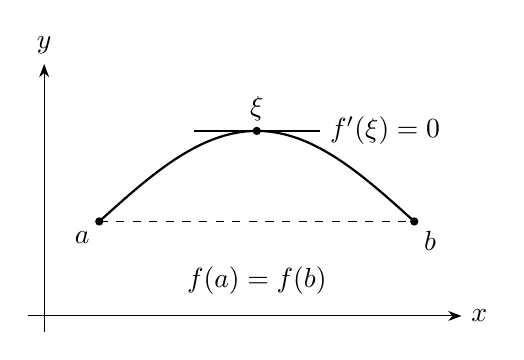
\begin{tikzpicture}[scale=1.0,>=Stealth]
  \draw[->] (-0.2,0)--(5.3,0) node[right] {$x$};
  \draw[->] (0,-0.2)--(0,3.2) node[above] {$y$};
  \draw[domain=0.7:4.7,smooth,variable=\x,thick]
    plot ({\x},{1.2+1.15*sin(45*(\x-0.7))});
  \coordinate (A) at (0.7,1.2);
  \coordinate (B) at (4.7,1.2);
  \coordinate (C) at (2.7,2.35);
  \fill (A) circle (1.5pt) node[below left] {$a$};
  \fill (B) circle (1.5pt) node[below right] {$b$};
  \fill (C) circle (1.5pt) node[above] {$\xi$};
  \draw[dashed] (A)--(B);
  \draw[thick] (1.9,2.35)--(3.5,2.35) node[right] {$f'(\xi)=0$};
  \node at (2.7,0.45) {$f(a)=f(b)$};
\end{tikzpicture}
\end{center}
% SOURCE-END U0008
}
\end{frame}
\typeout{MATH-AGENT-FRAME-END F005}
% FRAME-ID F006
\typeout{MATH-AGENT-FRAME-BEGIN F006}
\begin{frame}[t,fragile]{罗尔定理与拉格朗日中值定理}
\footnotesize
\begin{block}{定理}
{\footnotesize
% SOURCE-BEGIN U0009 0 120
\textbf{拉格朗日中值定理}\par

若 $f$ 在 $[a,b]$ 上连续，在 $(a,b)$ 内可导，则存在 $\xi\in(a,b)$，使得
\[
f'(\xi)=\frac{f(b)-f(a)}{b-a}.
\]

% SOURCE-END U0009
}
\end{block}
\pause
{\footnotesize
\textbf{证明：}
% SOURCE-BEGIN U0010 0 237
构造辅助函数
\[
F(x)=f(x)-\frac{f(b)-f(a)}{b-a}(x-a).
\]
$F$ 在 $[a,b]$ 上连续，在 $(a,b)$ 内可导，且
\[
F(a)=f(a),\qquad F(b)=f(b)-[f(b)-f(a)]=f(a).
\]
由罗尔定理，存在 $\xi\in(a,b)$ 使 $F'(\xi)=0$。 而
\[
F'(x)=f'(x)-\frac{f(b)-f(a)}{b-a},
\]
故结论成立。

% SOURCE-END U0010
}
\end{frame}
\typeout{MATH-AGENT-FRAME-END F006}
% FRAME-ID F007
\typeout{MATH-AGENT-FRAME-BEGIN F007}
\begin{frame}[t,fragile]{罗尔定理与拉格朗日中值定理}
\normalsize
{\normalsize
% SOURCE-BEGIN U0011 0 110
拉格朗日中值定理的几何意义是：连续光滑曲线上至少有一点的切线平行于连接两端点的弦。 公式
\[
f(b)-f(a)=f'(\xi)(b-a)
\]
说明“总改变量”等于某个中间点的瞬时变化率乘以区间长度。


% SOURCE-END U0011
}
\end{frame}
\typeout{MATH-AGENT-FRAME-END F007}
% FRAME-ID F008
\typeout{MATH-AGENT-FRAME-BEGIN F008}
\begin{frame}[t,fragile]{罗尔定理与拉格朗日中值定理}
\normalsize
{\normalsize
% PRESENTATION-SCAFFOLD isotropic coordinates; node font size unchanged
\tikzset{every picture/.append style={scale=0.75}}
% SOURCE-BEGIN U0012 0 1067
\begin{center}
\begin{tikzpicture}[scale=1.0,>=Stealth]
  \draw[->] (-0.2,0)--(5.4,0) node[right] {$x$};
  \draw[->] (0,-0.2)--(0,4.0) node[above] {$y$};
  % y=0.18(x-2.2)^2+1, with a=0.8, b=4.6.
  % The secant slope equals f'(2.7)=0.18, so the tangent at xi=2.7 is parallel to the secant.
  \draw[domain=0.55:4.85,smooth,variable=\x,thick]
    plot ({\x},{0.18*(\x-2.2)*(\x-2.2)+1});
  \coordinate (A) at (0.8,1.353);
  \coordinate (B) at (4.6,2.037);
  \coordinate (C) at (2.7,1.045);
  \fill (A) circle (1.5pt) node[below left] {$(a,f(a))$};
  \fill (B) circle (1.5pt) node[above right] {$(b,f(b))$};
  \fill (C) circle (1.5pt) node[below] {$(\xi,f(\xi))$};
  \draw[thick,dashed] (A)--(B) node[midway,above,sloped] {弦};
  \draw[thick] ($(C)+(-1.2,-0.216)$)--($(C)+(1.2,0.216)$) node[right] {切线};
  \draw[dashed] (0.8,0)--(0.8,1.353);
  \draw[dashed] (2.7,0)--(2.7,1.045);
  \draw[dashed] (4.6,0)--(4.6,2.037);
  \node[below] at (0.8,0) {$a$};
  \node[below] at (2.7,0) {$\xi$};
  \node[below] at (4.6,0) {$b$};
\end{tikzpicture}
\end{center}
% SOURCE-END U0012
}
\end{frame}
\typeout{MATH-AGENT-FRAME-END F008}
% FRAME-ID F009
\typeout{MATH-AGENT-FRAME-BEGIN F009}
\begin{frame}[t,fragile]{罗尔定理与拉格朗日中值定理}
\normalsize
\begin{block}{例题}
{\normalsize
% SOURCE-BEGIN U0013 0 67
\textbf{验证中值定理}\par

对 $f(x)=x^2$ 在 $[1,3]$ 上求满足拉格朗日中值定理的 $\xi$。

% SOURCE-END U0013
}
\end{block}
\pause
{\normalsize
\textbf{解：}
% SOURCE-BEGIN U0014 0 92
\[
\frac{f(3)-f(1)}{3-1}=\frac{9-1}{2}=4.
\]
因 $f'(x)=2x$，令 $2\xi=4$ 得 $\xi=2\in(1,3)$。

% SOURCE-END U0014
}
\end{frame}
\typeout{MATH-AGENT-FRAME-END F009}
% FRAME-ID F010
\typeout{MATH-AGENT-FRAME-BEGIN F010}
\begin{frame}[t,fragile]{罗尔定理与拉格朗日中值定理}
\small
\begin{block}{例题}
{\small
% SOURCE-BEGIN U0015 0 74
\textbf{罗尔定理的条件核查}\par

判断函数
\[
f(x)=|x|
\]
在区间 $[-1,1]$ 上能否应用罗尔定理。

% SOURCE-END U0015
}
\end{block}
\pause
{\small
\textbf{解：}
% SOURCE-BEGIN U0016 0 222
首先，
\[
f(-1)=1,\qquad f(1)=1,
\]
两端函数值相等，且 $f$ 在 $[-1,1]$ 上连续。 但是 $f$ 在 $x=0$ 处不可导，因为
\[
\lim_{h\to0+}\frac{|h|-0}{h}=1,\qquad
\lim_{h\to0-}\frac{|h|-0}{h}=-1,
\]
左右导数不相等。 因此 $f$ 不满足“在 $(-1,1)$ 内可导”的条件，不能应用罗尔定理。

% SOURCE-END U0016
}
{\small
% SOURCE-BEGIN U0017 0 92
\begin{warning}
罗尔定理的结论不是只由 $f(a)=f(b)$ 推出。 连续性和开区间可导性缺一不可，本题图像有尖点，正好破坏了可导性。
\end{warning}
% SOURCE-END U0017
}
\end{frame}
\typeout{MATH-AGENT-FRAME-END F010}
% FRAME-ID F011
\typeout{MATH-AGENT-FRAME-BEGIN F011}
\begin{frame}[t,fragile]{罗尔定理与拉格朗日中值定理}
\footnotesize
\begin{block}{例题}
{\footnotesize
% SOURCE-BEGIN U0018 0 78
\textbf{罗尔定理证明方程根的个数}\par

证明方程
\[
x^3-3x+1=0
\]
在区间 $(-2,2)$ 内有三个不同实根。

% SOURCE-END U0018
}
\end{block}
\pause
{\footnotesize
\textbf{解：}
% SOURCE-BEGIN U0019 0 443
设
\[
f(x)=x^3-3x+1.
\]
计算得
\[
f(-2)=-1,\quad f(-1)=3,\quad f(0)=1,\quad f(1)=-1,\quad f(2)=3.
\]
由介值定理，区间 $(-2,-1)$、$(0,1)$、$(1,2)$ 内各至少有一个零点，所以 $(-2,2)$ 内至少有三个不同实根。

下面证明不可能有四个或更多不同实根。 若存在四个不同实根
\[
r_1<r_2<r_3<r_4,
\]
则在每个区间 $[r_i,r_{i+1}]$ 上，函数连续、开区间内可导，且两端函数值都为 $0$。 由罗尔定理，$f'$ 在 $(r_1,r_2)$、$(r_2,r_3)$、$(r_3,r_4)$ 内各至少有一个零点，因此 $f'$ 至少有三个不同零点。 但
\[
f'(x)=3x^2-3=3(x-1)(x+1)
\]
只有两个零点 $-1,1$，矛盾。 故方程在 $(-2,2)$ 内恰有三个不同实根。

% SOURCE-END U0019
}
\end{frame}
\typeout{MATH-AGENT-FRAME-END F011}
% FRAME-ID F012
\typeout{MATH-AGENT-FRAME-BEGIN F012}
\begin{frame}[t,fragile]{罗尔定理与拉格朗日中值定理}
\footnotesize
\begin{block}{例题}
{\footnotesize
% SOURCE-BEGIN U0020 0 129
\textbf{构造辅助函数}\par

设 $f$ 在 $[0,1]$ 上连续，在 $(0,1)$ 内可导，且 $f(1)=0$。 证明存在 $\xi\in(0,1)$，使得
\[
f'(\xi)=-\frac{f(\xi)}{\xi}.
\]

% SOURCE-END U0020
}
\end{block}
\pause
{\footnotesize
\textbf{解：}
% SOURCE-BEGIN U0021 0 272
令
\[
F(x)=xf(x).
\]
则 $F$ 在 $[0,1]$ 上连续，在 $(0,1)$ 内可导，并且
\[
F(0)=0,\qquad F(1)=f(1)=0.
\]
由罗尔定理，存在 $\xi\in(0,1)$，使得 $F'(\xi)=0$。 而
\[
F'(x)=f(x)+xf'(x),
\]
所以
\[
f(\xi)+\xi f'(\xi)=0.
\]
由于 $\xi\in(0,1)$，可除以 $\xi$，得到
\[
f'(\xi)=-\frac{f(\xi)}{\xi}.
\]

% SOURCE-END U0021
}
\end{frame}
\typeout{MATH-AGENT-FRAME-END F012}
% FRAME-ID F013
\typeout{MATH-AGENT-FRAME-BEGIN F013}
\begin{frame}[t,fragile]{罗尔定理与拉格朗日中值定理}
\small
\begin{block}{例题}
{\small
% SOURCE-BEGIN U0022 0 123
\textbf{构造辅助函数}\par

设 $f$ 在 $[a,b]$ 上连续，在 $(a,b)$ 内可导，且 $f(a)=f(b)=0$。 证明存在 $\xi\in(a,b)$，使得
\[
f'(\xi)+f(\xi)=0.
\]

% SOURCE-END U0022
}
\end{block}
\pause
{\small
\textbf{解：}
% SOURCE-BEGIN U0023 0 315
观察到表达式 $f'(x)+f(x)$ 是 $\ee^x f(x)$ 的导数中除去正因子后的部分。 令
\[
F(x)=\ee^x f(x).
\]
则 $F$ 在 $[a,b]$ 上连续，在 $(a,b)$ 内可导，并且
\[
F(a)=\ee^a f(a)=0,\qquad F(b)=\ee^b f(b)=0.
\]
由罗尔定理，存在 $\xi\in(a,b)$，使得 $F'(\xi)=0$。 而
\[
F'(x)=\ee^x f(x)+\ee^x f'(x)=\ee^x[f'(x)+f(x)].
\]
由于 $\ee^\xi>0$，所以
\[
f'(\xi)+f(\xi)=0.
\]

% SOURCE-END U0023
}
\end{frame}
\typeout{MATH-AGENT-FRAME-END F013}
% FRAME-ID F014
\typeout{MATH-AGENT-FRAME-BEGIN F014}
\begin{frame}[t,fragile]{罗尔定理与拉格朗日中值定理}
\small
\begin{block}{例题}
{\small
% SOURCE-BEGIN U0024 0 185
\textbf{由导数界估计函数增量}\par

设 $f$ 在 $[a,b]$ 上连续，在 $(a,b)$ 内可导，且存在常数 $M>0$，使得
\[
|f'(x)|\leq M,\qquad x\in(a,b).
\]
证明对任意 $x_1,x_2\in[a,b]$，有
\[
|f(x_2)-f(x_1)|\leq M|x_2-x_1|.
\]

% SOURCE-END U0024
}
\end{block}
\pause
{\small
\textbf{解：}
% SOURCE-BEGIN U0025 0 198
若 $x_1=x_2$，结论成立。 设 $x_1<x_2$。 由拉格朗日中值定理，存在 $\xi\in(x_1,x_2)$，使得
\[
f(x_2)-f(x_1)=f'(\xi)(x_2-x_1).
\]
取绝对值得
\[
|f(x_2)-f(x_1)|=|f'(\xi)|\,|x_2-x_1|\leq M|x_2-x_1|.
\]
当 $x_1>x_2$ 时交换两点即可。

% SOURCE-END U0025
}
\end{frame}
\typeout{MATH-AGENT-FRAME-END F014}
% FRAME-ID F015
\typeout{MATH-AGENT-FRAME-BEGIN F015}
\begin{frame}[t,fragile]{罗尔定理与拉格朗日中值定理}
\normalsize
{\normalsize
% SOURCE-BEGIN U0026 0 343
\begin{application}[物理：平均速度与瞬时速度]
设质点位置为 $s(t)$，单位分别为 $[s]=\mathrm m$、$[t]=\mathrm s$。若 $s$ 在 $[t_1,t_2]$ 上连续、在 $(t_1,t_2)$ 内可导，则拉格朗日中值定理保证存在 $\xi\in(t_1,t_2)$，使
\[
s'(\xi)=\frac{s(t_2)-s(t_1)}{t_2-t_1}.
\]
左边是时刻 $\xi$ 的瞬时速度，右边是该时间段的平均速度，二者单位均为 $\mathrm{m/s}$。因此，一段时间内的平均速度会在某个中间时刻真正取到。这里要求位置函数可导；若运动发生瞬时跳变，这一结论的条件便不满足。
\end{application}
% SOURCE-END U0026
}
\end{frame}
\typeout{MATH-AGENT-FRAME-END F015}
% FRAME-ID F016
\typeout{MATH-AGENT-FRAME-BEGIN F016}
\begin{frame}[t,fragile]{罗尔定理与拉格朗日中值定理}
\normalsize
{\normalsize
% SOURCE-BEGIN U0027 0 343
\begin{application}[工程：传感器误差上界]
设温度传感器的标定函数为 $V(T)$，并假设在工作区间内
\[
|V'(T)|\leq0.02\ \mathrm{V/^{\circ}C}.
\]
若输入温度误差满足 $|\Delta T|\leq0.5\,^{\circ}\mathrm C$，则由中值定理，存在中间温度 $\xi$ 使
\[
|\Delta V|=|V'(\xi)|\,|\Delta T|
\leq0.02\times0.5
=0.01\ \mathrm V.
\]
这个估计把“灵敏度上界”转化为“输出误差上界”。它只计入由温度输入误差引起的变化；零点漂移、噪声等其他误差需要另行分析。
\end{application}
% SOURCE-END U0027
}
\end{frame}
\typeout{MATH-AGENT-FRAME-END F016}
\section{柯西中值定理与若干推论}
% FRAME-ID F017
\typeout{MATH-AGENT-FRAME-BEGIN F017}
\begin{frame}[t,fragile]{目录}
\normalsize
{\color{black}\normalsize 1. 罗尔定理与拉格朗日中值定理\par}\vspace{0.22em}
{\color{blue}\normalsize 2. 柯西中值定理与若干推论\par}\vspace{0.22em}
{\color{gray!40}\normalsize 3. 洛必达法则\par}\vspace{0.22em}
{\color{gray!40}\normalsize 4. 函数单调性判别法\par}\vspace{0.22em}
{\color{gray!40}\normalsize 5. 函数的极值\par}\vspace{0.22em}
{\color{gray!40}\normalsize 6. 函数的最值与应用优化\par}\vspace{0.22em}
{\color{gray!40}\normalsize 7. 曲线的凸性与拐点\par}\vspace{0.22em}
{\color{gray!40}\normalsize 8. 曲线的渐近线与函数图像\par}\vspace{0.22em}
{\color{gray!40}\normalsize 9. 泰勒公式\par}\vspace{0.22em}
\end{frame}
\typeout{MATH-AGENT-FRAME-END F017}
% FRAME-ID F018
\typeout{MATH-AGENT-FRAME-BEGIN F018}
\begin{frame}[t,fragile]{柯西中值定理与若干推论}
\small
\begin{block}{定理}
{\small
% SOURCE-BEGIN U0028 0 176
\textbf{柯西中值定理}\par

若 $f,g$ 在 $[a,b]$ 上连续，在 $(a,b)$ 内可导，且 $g'(x)\neq0$ 对所有 $x\in(a,b)$ 成立，则存在 $\xi\in(a,b)$，使得
\[
\frac{f'(\xi)}{g'(\xi)}=\frac{f(b)-f(a)}{g(b)-g(a)}.
\]

% SOURCE-END U0028
}
\end{block}
\pause
{\small
\textbf{证明：}
% SOURCE-BEGIN U0029 0 332
先说明 $g(b)\neq g(a)$。 若 $g(b)=g(a)$，由罗尔定理存在 $\eta\in(a,b)$ 使 $g'(\eta)=0$，与条件矛盾。

构造
\[
F(x)=f(x)-f(a)-\frac{f(b)-f(a)}{g(b)-g(a)}[g(x)-g(a)].
\]
则 $F$ 在 $[a,b]$ 连续，在 $(a,b)$ 可导，且 $F(a)=F(b)=0$。 由罗尔定理，存在 $\xi\in(a,b)$ 使 $F'(\xi)=0$。 即
\[
f'(\xi)-\frac{f(b)-f(a)}{g(b)-g(a)}g'(\xi)=0.
\]
因 $g'(\xi)\neq0$，除以 $g'(\xi)$ 得结论。

% SOURCE-END U0029
}
\end{frame}
\typeout{MATH-AGENT-FRAME-END F018}
% FRAME-ID F019
\typeout{MATH-AGENT-FRAME-BEGIN F019}
\begin{frame}[t,fragile]{柯西中值定理与若干推论}
\normalsize
\begin{block}{命题}
{\normalsize
% SOURCE-BEGIN U0030 0 92
\textbf{导数恒为零的函数为常数}\par

若 $f$ 在区间 $I$ 上可导，且 $f'(x)=0$ 对所有 $x\in I$ 成立，则 $f$ 在 $I$ 上为常数。

% SOURCE-END U0030
}
\end{block}
\pause
{\normalsize
\textbf{证明：}
% SOURCE-BEGIN U0031 0 169
任取 $x_1,x_2\in I$，不妨 $x_1<x_2$。 $f$ 在 $[x_1,x_2]$ 连续、在 $(x_1,x_2)$ 可导。 由拉格朗日中值定理，存在 $\xi\in(x_1,x_2)$ 使
\[
f(x_2)-f(x_1)=f'(\xi)(x_2-x_1)=0.
\]
故任意两点函数值相等，$f$ 为常数。

% SOURCE-END U0031
}
\end{frame}
\typeout{MATH-AGENT-FRAME-END F019}
% FRAME-ID F020
\typeout{MATH-AGENT-FRAME-BEGIN F020}
\begin{frame}[t,fragile]{柯西中值定理与若干推论}
\normalsize
\begin{block}{命题}
{\normalsize
% SOURCE-BEGIN U0032 0 136
\textbf{导数相等的函数相差常数}\par

若 $f,g$ 在区间 $I$ 上可导，且
\[
f'(x)=g'(x),\qquad x\in I,
\]
则存在常数 $C$，使得
\[
f(x)=g(x)+C,\qquad x\in I.
\]

% SOURCE-END U0032
}
\end{block}
\pause
{\normalsize
\textbf{证明：}
% SOURCE-BEGIN U0033 0 119
令 $h(x)=f(x)-g(x)$。 则 $h$ 在 $I$ 上可导，且
\[
h'(x)=f'(x)-g'(x)=0.
\]
由“导数恒为零的函数为常数”，$h(x)=C$。 即
\[
f(x)-g(x)=C.
\]

% SOURCE-END U0033
}
\end{frame}
\typeout{MATH-AGENT-FRAME-END F020}
% FRAME-ID F021
\typeout{MATH-AGENT-FRAME-BEGIN F021}
\begin{frame}[t,fragile]{柯西中值定理与若干推论}
\small
\begin{block}{例题}
{\small
% SOURCE-BEGIN U0034 0 99
\textbf{柯西中值定理验证}\par

设
\[
f(x)=\ln x,\qquad g(x)=x,\qquad x\in[1,\ee].
\]
求柯西中值定理中的 $\xi$。

% SOURCE-END U0034
}
\end{block}
\pause
{\small
\textbf{解：}
% SOURCE-BEGIN U0035 0 266
$f,g$ 在 $[1,\ee]$ 上连续，在 $(1,\ee)$ 内可导，且 $g'(x)=1\neq0$。柯西中值定理给出存在 $\xi\in(1,\ee)$，使
\[
\frac{f'(\xi)}{g'(\xi)}
=\frac{f(\ee)-f(1)}{g(\ee)-g(1)}.
\]
即
\[
\frac{1/\xi}{1}=\frac{1-0}{\ee-1}=\frac1{\ee-1}.
\]
因此
\[
\xi=\ee-1.
\]
由于 $1<\ee-1<\ee$，该点确在区间内部。

% SOURCE-END U0035
}
\end{frame}
\typeout{MATH-AGENT-FRAME-END F021}
% FRAME-ID F022
\typeout{MATH-AGENT-FRAME-BEGIN F022}
\begin{frame}[t,fragile]{柯西中值定理与若干推论}
\small
\begin{block}{例题}
{\small
% SOURCE-BEGIN U0036 0 94
\textbf{用柯西中值定理证明不等式}\par

证明当 $0<a<b$ 时，
\[
\frac{b-a}{b}<\ln b-\ln a<\frac{b-a}{a}.
\]

% SOURCE-END U0036
}
\end{block}
\pause
{\small
\textbf{解：}
% SOURCE-BEGIN U0037 0 265
对 $f(x)=\ln x$ 和 $g(x)=x$ 在 $[a,b]$ 上应用柯西中值定理，存在 $\xi\in(a,b)$，使得
\[
\frac{\ln b-\ln a}{b-a}=\frac{f'(\xi)}{g'(\xi)}=\frac1{\xi}.
\]
因为 $a<\xi<b$，所以
\[
\frac1b<\frac1\xi<\frac1a.
\]
又 $b-a>0$，两边同乘以 $b-a$ 得
\[
\frac{b-a}{b}<\ln b-\ln a<\frac{b-a}{a}.
\]

% SOURCE-END U0037
}
\end{frame}
\typeout{MATH-AGENT-FRAME-END F022}
% FRAME-ID F023
\typeout{MATH-AGENT-FRAME-BEGIN F023}
\begin{frame}[t,fragile]{柯西中值定理与若干推论}
\normalsize
\begin{block}{例题}
{\normalsize
% SOURCE-BEGIN U0038 0 46
\textbf{不等式}\par

证明当 $x>0$ 时，$\ln(1+x)<x$。

% SOURCE-END U0038
}
\end{block}
\pause
{\normalsize
\textbf{解：}
% SOURCE-BEGIN U0039 0 158
令 $f(t)=\ln(1+t)$，在 $[0,x]$ 上应用拉格朗日中值定理，存在 $\xi\in(0,x)$ 使
\[
\ln(1+x)-\ln1=f'(\xi)x=\frac{x}{1+\xi}.
\]
因 $\xi>0$，有 $1+\xi>1$，故 $\ln(1+x)=x/(1+\xi)<x$。

% SOURCE-END U0039
}
\end{frame}
\typeout{MATH-AGENT-FRAME-END F023}
% FRAME-ID F024
\typeout{MATH-AGENT-FRAME-BEGIN F024}
\begin{frame}[t,fragile]{柯西中值定理与若干推论}
\footnotesize
\begin{block}{例题}
{\footnotesize
% SOURCE-BEGIN U0040 0 66
\textbf{不等式}\par

证明当 $x>0$ 时，
\[
\ln(1+x)>\frac{x}{1+x}.
\]

% SOURCE-END U0040
}
\end{block}
\pause
{\footnotesize
\textbf{解：}
% SOURCE-BEGIN U0041 0 248
令
\[
F(x)=\ln(1+x)-\frac{x}{1+x},\qquad x\geq0.
\]
有 $F(0)=0$，且当 $x>0$ 时
\[
F'(x)=\frac1{1+x}-\frac1{(1+x)^2}
=\frac{x}{(1+x)^2}>0.
\]
由单调性判别法，$F$ 在 $[0,\infty)$ 上单调增加。 因此对 $x>0$，
\[
F(x)>F(0)=0,
\]
即
\[
\ln(1+x)>\frac{x}{1+x}.
\]

% SOURCE-END U0041
}
\end{frame}
\typeout{MATH-AGENT-FRAME-END F024}
% FRAME-ID F025
\typeout{MATH-AGENT-FRAME-BEGIN F025}
\begin{frame}[t,fragile]{柯西中值定理与若干推论}
\normalsize
\begin{block}{例题}
{\normalsize
% SOURCE-BEGIN U0042 0 56
\textbf{三角函数不等式}\par

证明当 $x>0$ 时，
\[
\sin x<x.
\]

% SOURCE-END U0042
}
\end{block}
\pause
{\normalsize
\textbf{解：}
% SOURCE-BEGIN U0043 0 220
当 $x\geq\pi$ 时，$\sin x\leq1<x$，结论成立。 下面只需考虑 $0<x<\pi$。

令 $f(t)=\sin t$，在 $[0,x]$ 上应用拉格朗日中值定理，存在 $\xi\in(0,x)$，使得
\[
\sin x-\sin0=f'(\xi)x=\cos\xi\,x.
\]
由于 $0<\xi<\pi$，有 $\cos\xi<1$，故
\[
\sin x=x\cos\xi<x.
\]

% SOURCE-END U0043
}
\end{frame}
\typeout{MATH-AGENT-FRAME-END F025}
% FRAME-ID F026
\typeout{MATH-AGENT-FRAME-BEGIN F026}
\begin{frame}[t,fragile]{柯西中值定理与若干推论}
\small
\begin{block}{例题}
{\small
% SOURCE-BEGIN U0044 0 76
\textbf{指数函数不等式}\par

证明对一切实数 $x$，
\[
\ee^x\geq1+x,
\]
且等号当且仅当 $x=0$。

% SOURCE-END U0044
}
\end{block}
\pause
{\small
\textbf{解：}
% SOURCE-BEGIN U0045 0 268
令
\[
F(x)=\ee^x-1-x.
\]
则
\[
F'(x)=\ee^x-1.
\]
当 $x<0$ 时，$F'(x)<0$；当 $x>0$ 时，$F'(x)>0$。 因而 $F$ 在 $(-\infty,0)$ 上单调减少，在 $(0,\infty)$ 上单调增加，所以 $x=0$ 是全局最小点。 又
\[
F(0)=0.
\]
于是 $F(x)\geq0$，即
\[
\ee^x\geq1+x.
\]
当 $x\neq0$ 时，$F(x)>F(0)=0$，故等号仅当 $x=0$ 成立。

% SOURCE-END U0045
}
\end{frame}
\typeout{MATH-AGENT-FRAME-END F026}
\section{洛必达法则}
% FRAME-ID F027
\typeout{MATH-AGENT-FRAME-BEGIN F027}
\begin{frame}[t,fragile]{目录}
\normalsize
{\color{black}\normalsize 1. 罗尔定理与拉格朗日中值定理\par}\vspace{0.22em}
{\color{black}\normalsize 2. 柯西中值定理与若干推论\par}\vspace{0.22em}
{\color{blue}\normalsize 3. 洛必达法则\par}\vspace{0.22em}
{\color{gray!40}\normalsize 4. 函数单调性判别法\par}\vspace{0.22em}
{\color{gray!40}\normalsize 5. 函数的极值\par}\vspace{0.22em}
{\color{gray!40}\normalsize 6. 函数的最值与应用优化\par}\vspace{0.22em}
{\color{gray!40}\normalsize 7. 曲线的凸性与拐点\par}\vspace{0.22em}
{\color{gray!40}\normalsize 8. 曲线的渐近线与函数图像\par}\vspace{0.22em}
{\color{gray!40}\normalsize 9. 泰勒公式\par}\vspace{0.22em}
\end{frame}
\typeout{MATH-AGENT-FRAME-END F027}
% FRAME-ID F028
\typeout{MATH-AGENT-FRAME-BEGIN F028}
\begin{frame}[t,fragile]{洛必达法则}
\footnotesize
\begin{block}{定理}
{\footnotesize
% SOURCE-BEGIN U0046 0 265
\textbf{洛必达法则：$0/0$ 型}\par

设 $f,g$ 在 $a$ 的某去心右邻域内可导，且 $g'(x)\neq0$。 若
\[
\lim_{x\to a+}f(x)=\lim_{x\to a+}g(x)=0,\qquad
\lim_{x\to a+}\frac{f'(x)}{g'(x)}=L
\]
其中 $L$ 可为有限数或无穷大，则
\[
\lim_{x\to a+}\frac{f(x)}{g(x)}=L.
\]
左极限、双侧极限与 $x\to\infty$ 的相应形式类似成立。

% SOURCE-END U0046
}
\end{block}
\end{frame}
\typeout{MATH-AGENT-FRAME-END F028}
% FRAME-ID F029
\typeout{MATH-AGENT-FRAME-BEGIN F029}
\begin{frame}[t,fragile]{洛必达法则}
\footnotesize
{\footnotesize
\textbf{证明：}
% SOURCE-BEGIN U0047 0 803
先证 $L$ 为有限数的情形。 任取 $\varepsilon>0$，由 $\frac{f'}{g'}\to L$，存在 $\delta>0$，当 $a<x<a+\delta$ 时，
\[
L-\varepsilon<\frac{f'(x)}{g'(x)}<L+\varepsilon.
\]
取 $x\in(a,a+\delta)$，再取 $t\in(a,x)$。 在 $[t,x]$ 上对 $f,g$ 应用柯西中值定理，存在 $\xi\in(t,x)$ 使
\[
\frac{f(x)-f(t)}{g(x)-g(t)}=\frac{f'(\xi)}{g'(\xi)}.
\]
因此
\[
\left|\frac{f(x)-f(t)}{g(x)-g(t)}-L\right|<\varepsilon.
\]
固定 $x$ 后令 $t\to a+$，由 $f(t)\to0,g(t)\to0$ 得
\[
\left|\frac{f(x)}{g(x)}-L\right|\leq\varepsilon
\]
其中 $x\in(a,a+\delta)$ 且 $g(x)\neq0$。 因 $\varepsilon$ 任意，得 $\frac{f(x)}{g(x)}\to L$。

若 $L=+\infty$，任取 $M>0$，可令 $\delta>0$ 充分小，使 $a<x<a+\delta$ 时 $\frac{f'(x)}{g'(x)}>2M$。重复上面的柯西中值定理步骤，先得到相应差商大于 $2M$，再令 $t\to a+$，可得 $\frac{f(x)}{g(x)}\geq2M>M$，故极限为 $+\infty$。若 $L=-\infty$，同理使用 $\frac{f'}{g'}<-2M$，得到 $\frac{f(x)}{g(x)}\leq-2M<-M$。

% SOURCE-END U0047
}
\end{frame}
\typeout{MATH-AGENT-FRAME-END F029}
% FRAME-ID F030
\typeout{MATH-AGENT-FRAME-BEGIN F030}
\begin{frame}[t,fragile]{洛必达法则}
\footnotesize
\begin{block}{定理}
{\footnotesize
% SOURCE-BEGIN U0048 0 308
\textbf{洛必达法则：$\infty/\infty$ 型}\par

设 $f,g$ 在 $a$ 的某去心右邻域内可导，且 $g'(x)\neq0$。 若
\[
\lim_{x\to a+}|f(x)|=+\infty,\qquad
\lim_{x\to a+}|g(x)|=+\infty,
\]
并且
\[
\lim_{x\to a+}\frac{f'(x)}{g'(x)}=L,
\]
其中 $L$ 可为有限数或无穷大，则
\[
\lim_{x\to a+}\frac{f(x)}{g(x)}=L.
\]
左极限、双侧极限与 $x\to\infty$ 的相应形式类似成立。

% SOURCE-END U0048
}
\end{block}
\end{frame}
\typeout{MATH-AGENT-FRAME-END F030}
% FRAME-ID F031
\typeout{MATH-AGENT-FRAME-BEGIN F031}
\begin{frame}[t,fragile]{洛必达法则}
\footnotesize
{\footnotesize
\textbf{证明：}
% SOURCE-BEGIN U0049 0 643
证明有限 \(L\) 的情形。任取 \(\varepsilon>0\)，由 \(\frac{f'}{g'}\to L\)，存在 \(\delta>0\)，使得任意 \(u\in(a,a+\delta)\) 都满足
\[
\left|\frac{f'(u)}{g'(u)}-L\right|<\varepsilon.
\]
固定 \(x_0\in(a,a+\delta)\)。对任意 \(x\in(a,x_0)\)，在 \([x,x_0]\) 上应用柯西中值定理，存在 \(\xi\in(x,x_0)\subset(a,a+\delta)\)，使
\[
\frac{f(x)-f(x_0)}{g(x)-g(x_0)}=\frac{f'(\xi)}{g'(\xi)}.
\]
因此
\[
\left|\frac{f(x)-f(x_0)}{g(x)-g(x_0)}-L\right|<\varepsilon.
\]
另一方面，
\[
\frac{f(x)}{g(x)}
=\frac{f(x)-f(x_0)}{g(x)-g(x_0)}
\left(1-\frac{g(x_0)}{g(x)}\right)
+\frac{f(x_0)}{g(x)}.
\]
当 \(x\to a+\) 时，后两个因子分别趋于 \(1\) 和 \(0\)。由上式与 \(\varepsilon\) 的任意性可得 \(\frac{f(x)}{g(x)}\to L\)。


% SOURCE-END U0049
}
\end{frame}
\typeout{MATH-AGENT-FRAME-END F031}
% FRAME-ID F032
\typeout{MATH-AGENT-FRAME-BEGIN F032}
\begin{frame}[t,fragile]{洛必达法则（续1）}
\footnotesize
{\footnotesize
\textbf{证明：}
% SOURCE-BEGIN U0049 643 950
若 \(L=+\infty\)，任取 \(M>0\)，令 \(x\) 充分接近 \(a\)，使柯西中值定理给出的差商大于 \(4M\)，并且
\[
1-\frac{g(x_0)}{g(x)}>\frac12,
\qquad
\left|\frac{f(x_0)}{g(x)}\right|<M.
\]
代入上式即得 \(\frac{f(x)}{g(x)}>4M\cdot\frac12-M=M\)，所以 \(\frac{f(x)}{g(x)}\to+\infty\)。若 \(L=-\infty\)，使用差商小于 \(-4M\) 的同样估计，可得 \(\frac{f(x)}{g(x)}<-M\)。

% SOURCE-END U0049
}
\end{frame}
\typeout{MATH-AGENT-FRAME-END F032}
% FRAME-ID F033
\typeout{MATH-AGENT-FRAME-BEGIN F033}
\begin{frame}[t,fragile]{洛必达法则}
\footnotesize
{\footnotesize
% SOURCE-BEGIN U0050 0 154
\begin{warning}
洛必达法则只给出一组充分条件，不能反向使用。即使 \(\lim f(x)/g(x)\) 存在，\(\lim f'(x)/g'(x)\) 也可能不存在；使用法则前还必须先确认原式确为 \(0/0\) 型或 \(\infty/\infty\) 型。
\end{warning}
% SOURCE-END U0050
}
\end{frame}
\typeout{MATH-AGENT-FRAME-END F033}
% FRAME-ID F034
\typeout{MATH-AGENT-FRAME-BEGIN F034}
\begin{frame}[t,fragile]{洛必达法则}
\normalsize
\begin{block}{例题}
{\normalsize
% SOURCE-BEGIN U0051 0 71
\textbf{$0/0$ 型}\par

求 $\displaystyle\lim_{x\to0}\frac{\sin x}{x}$。

% SOURCE-END U0051
}
\end{block}
\pause
{\normalsize
\textbf{解：}
% SOURCE-BEGIN U0052 0 91
这是 $0/0$ 型。 用洛必达法则：
\[
\lim_{x\to0}\frac{\sin x}{x}=\lim_{x\to0}\frac{\cos x}{1}=1.
\]

% SOURCE-END U0052
}
\end{frame}
\typeout{MATH-AGENT-FRAME-END F034}
% FRAME-ID F035
\typeout{MATH-AGENT-FRAME-BEGIN F035}
\begin{frame}[t,fragile]{洛必达法则}
\normalsize
\begin{block}{例题}
{\normalsize
% SOURCE-BEGIN U0053 0 73
\textbf{多次使用}\par

求 $\displaystyle\lim_{x\to0}\frac{\ee^x-1-x}{x^2}$。

% SOURCE-END U0053
}
\end{block}
\pause
{\normalsize
\textbf{解：}
% SOURCE-BEGIN U0054 0 153
第一次洛必达：
\[
\lim_{x\to0}\frac{\ee^x-1-x}{x^2}
=\lim_{x\to0}\frac{\ee^x-1}{2x}.
\]
仍为 $0/0$ 型，第二次洛必达：
\[
=\lim_{x\to0}\frac{\ee^x}{2}=\frac12.
\]

% SOURCE-END U0054
}
{\normalsize
% SOURCE-BEGIN U0055 0 92
\begin{warning}
使用洛必达前必须确认是 $0/0$ 或 $\infty/\infty$ 型，并确认分母导数不为零的条件在去心邻域内成立。
\end{warning}
% SOURCE-END U0055
}
\end{frame}
\typeout{MATH-AGENT-FRAME-END F035}
% FRAME-ID F036
\typeout{MATH-AGENT-FRAME-BEGIN F036}
\begin{frame}[t,fragile]{洛必达法则}
\normalsize
\begin{block}{例题}
{\normalsize
% SOURCE-BEGIN U0056 0 102
\textbf{$\infty/\infty$ 型}\par

求
\[
\lim_{x\to\infty}\frac{\ln x}{x^\alpha},\qquad \alpha>0.
\]

% SOURCE-END U0056
}
\end{block}
\pause
{\normalsize
\textbf{解：}
% SOURCE-BEGIN U0057 0 253
当 $x\to\infty$ 时，分子、分母都趋于 $+\infty$，属于 $\infty/\infty$ 型。 用洛必达法则：
\[
\lim_{x\to\infty}\frac{\ln x}{x^\alpha}
=\lim_{x\to\infty}\frac{1/x}{\alpha x^{\alpha-1}}
=\lim_{x\to\infty}\frac{1}{\alpha x^\alpha}=0.
\]
这说明任意正幂函数 $x^\alpha$ 的增长都快于 $\ln x$。

% SOURCE-END U0057
}
\end{frame}
\typeout{MATH-AGENT-FRAME-END F036}
% FRAME-ID F037
\typeout{MATH-AGENT-FRAME-BEGIN F037}
\begin{frame}[t,fragile]{洛必达法则}
\normalsize
\begin{block}{例题}
{\normalsize
% SOURCE-BEGIN U0058 0 70
\textbf{三角函数高阶小量}\par

求
\[
\lim_{x\to0}\frac{\tan x-x}{x^3}.
\]

% SOURCE-END U0058
}
\end{block}
\pause
{\normalsize
\textbf{解：}
% SOURCE-BEGIN U0059 0 229
这是 $0/0$ 型。 第一次洛必达：
\[
\lim_{x\to0}\frac{\tan x-x}{x^3}
=\lim_{x\to0}\frac{\sec^2x-1}{3x^2}
=\lim_{x\to0}\frac{\tan^2x}{3x^2}.
\]
因为 $\lim_{x\to0}\frac{\tan x}{x}=1$，所以
\[
\lim_{x\to0}\frac{\tan^2x}{3x^2}
=\frac13.
\]

% SOURCE-END U0059
}
\end{frame}
\typeout{MATH-AGENT-FRAME-END F037}
% FRAME-ID F038
\typeout{MATH-AGENT-FRAME-BEGIN F038}
\begin{frame}[t,fragile]{洛必达法则}
\small
\begin{block}{例题}
{\small
% SOURCE-BEGIN U0060 0 90
\textbf{不能机械使用洛必达法则}\par

讨论 $\displaystyle\lim_{x\to\infty}\frac{x+\sin x}{x+\cos x}$。

% SOURCE-END U0060
}
\end{block}
\pause
{\small
\textbf{解：}
% SOURCE-BEGIN U0061 0 281
这是 $\infty/\infty$ 型，但直接看导数之比会得到
\[
\frac{(x+\sin x)'}{(x+\cos x)'}=\frac{1+\cos x}{1-\sin x},
\]
该式当 $x\to\infty$ 时无极限，因此不能由洛必达法则推出原极限不存在。 原式应先整理：
\[
\frac{x+\sin x}{x+\cos x}
=\frac{1+\frac{\sin x}{x}}{1+\frac{\cos x}{x}}.
\]
由于 $\sin x/x\to0,\ \cos x/x\to0$，原极限为 $1$。

% SOURCE-END U0061
}
{\small
% SOURCE-BEGIN U0062 0 87
\begin{warning}
洛必达法则给出的是充分条件：若导数之比的极限存在，原比值极限等于它。 导数之比极限不存在时，原极限仍可能存在。
\end{warning}
% SOURCE-END U0062
}
\end{frame}
\typeout{MATH-AGENT-FRAME-END F038}
% FRAME-ID F039
\typeout{MATH-AGENT-FRAME-BEGIN F039}
\begin{frame}[t,fragile]{洛必达法则}
\normalsize
\begin{block}{例题}
{\normalsize
% SOURCE-BEGIN U0063 0 60
\textbf{转化未定式}\par

求 $\displaystyle\lim_{x\to0+}x\ln x$。

% SOURCE-END U0063
}
\end{block}
\pause
{\normalsize
\textbf{解：}
% SOURCE-BEGIN U0064 0 204
原式为 $0\cdot(-\infty)$ 型，改写为
\[
x\ln x=\frac{\ln x}{1/x}.
\]
当 $x\to0+$ 时为 $-\infty/\infty$ 型。 用洛必达法则：
\[
\lim_{x\to0+}\frac{\ln x}{1/x}
=\lim_{x\to0+}\frac{1/x}{-1/x^2}
=\lim_{x\to0+}(-x)=0.
\]

% SOURCE-END U0064
}
\end{frame}
\typeout{MATH-AGENT-FRAME-END F039}
% FRAME-ID F040
\typeout{MATH-AGENT-FRAME-BEGIN F040}
\begin{frame}[t,fragile]{洛必达法则}
\footnotesize
\begin{block}{例题}
{\footnotesize
% SOURCE-BEGIN U0065 0 52
\textbf{指数型未定式}\par

求
\[
\lim_{x\to0+}x^x.
\]

% SOURCE-END U0065
}
\end{block}
\pause
{\footnotesize
\textbf{解：}
% SOURCE-BEGIN U0066 0 181
原式为 $0^0$ 型。 设
\[
y=x^x.
\]
取对数得
\[
\ln y=x\ln x.
\]
由上一例，
\[
\lim_{x\to0+}x\ln x=0.
\]
因此
\[
\lim_{x\to0+}\ln y=0.
\]
由于指数函数连续，
\[
\lim_{x\to0+}x^x=\ee^0=1.
\]

% SOURCE-END U0066
}
\end{frame}
\typeout{MATH-AGENT-FRAME-END F040}
% FRAME-ID F041
\typeout{MATH-AGENT-FRAME-BEGIN F041}
\begin{frame}[t,fragile]{洛必达法则}
\small
\begin{block}{例题}
{\small
% SOURCE-BEGIN U0067 0 84
\textbf{差型未定式}\par

求
\[
\lim_{x\to0+}\left(\frac1x-\frac1{\ee^x-1}\right).
\]

% SOURCE-END U0067
}
\end{block}
\pause
{\small
\textbf{解：}
% SOURCE-BEGIN U0068 0 306
原式为 $\infty-\infty$ 型，先通分：
\[
\frac1x-\frac1{\ee^x-1}
=\frac{\ee^x-1-x}{x(\ee^x-1)}.
\]
当 $x\to0+$ 时为 $0/0$ 型。 用洛必达法则：
\[
\lim_{x\to0+}\frac{\ee^x-1-x}{x(\ee^x-1)}
=\lim_{x\to0+}\frac{\ee^x-1}{\ee^x-1+x\ee^x}.
\]
仍为 $0/0$ 型，再用一次洛必达：
\[
=\lim_{x\to0+}\frac{\ee^x}{2\ee^x+x\ee^x}
=\frac12.
\]

% SOURCE-END U0068
}
\end{frame}
\typeout{MATH-AGENT-FRAME-END F041}
% FRAME-ID F042
\typeout{MATH-AGENT-FRAME-BEGIN F042}
\begin{frame}[t,fragile]{洛必达法则}
\normalsize
\begin{block}{例题}
{\normalsize
% SOURCE-BEGIN U0069 0 71
\textbf{参数型极限}\par

设 $a>0$。 求
\[
\lim_{x\to0}\frac{a^x-1}{x}.
\]

% SOURCE-END U0069
}
\end{block}
\pause
{\normalsize
\textbf{解：}
% SOURCE-BEGIN U0070 0 172
当 $x\to0$ 时为 $0/0$ 型。 由洛必达法则，
\[
\lim_{x\to0}\frac{a^x-1}{x}
=\lim_{x\to0}\frac{a^x\ln a}{1}
=\ln a.
\]
特别地，当 $a=\ee$ 时，得到
\[
\lim_{x\to0}\frac{\ee^x-1}{x}=1.
\]

% SOURCE-END U0070
}
\end{frame}
\typeout{MATH-AGENT-FRAME-END F042}
\section{函数单调性判别法}
% FRAME-ID F043
\typeout{MATH-AGENT-FRAME-BEGIN F043}
\begin{frame}[t,fragile]{目录}
\normalsize
{\color{black}\normalsize 1. 罗尔定理与拉格朗日中值定理\par}\vspace{0.22em}
{\color{black}\normalsize 2. 柯西中值定理与若干推论\par}\vspace{0.22em}
{\color{black}\normalsize 3. 洛必达法则\par}\vspace{0.22em}
{\color{blue}\normalsize 4. 函数单调性判别法\par}\vspace{0.22em}
{\color{gray!40}\normalsize 5. 函数的极值\par}\vspace{0.22em}
{\color{gray!40}\normalsize 6. 函数的最值与应用优化\par}\vspace{0.22em}
{\color{gray!40}\normalsize 7. 曲线的凸性与拐点\par}\vspace{0.22em}
{\color{gray!40}\normalsize 8. 曲线的渐近线与函数图像\par}\vspace{0.22em}
{\color{gray!40}\normalsize 9. 泰勒公式\par}\vspace{0.22em}
\end{frame}
\typeout{MATH-AGENT-FRAME-END F043}
% FRAME-ID F044
\typeout{MATH-AGENT-FRAME-BEGIN F044}
\begin{frame}[t,fragile]{函数单调性判别法}
\normalsize
\begin{block}{定理}
{\normalsize
% SOURCE-BEGIN U0071 0 182
\textbf{单调性判别法}\par

设 $f$ 在区间 $I$ 上连续，在 $I$ 的内部可导。 若 $f'(x)\geq0$ 对内部所有点成立，则 $f$ 在 $I$ 上单调不减；若 $f'(x)>0$ 对内部所有点成立，则 $f$ 在 $I$ 上严格单调增加。 相应地，$f'(x)\leq0$ 推出单调不增，$f'(x)<0$ 推出严格单调减少。

% SOURCE-END U0071
}
\end{block}
\pause
{\normalsize
\textbf{证明：}
% SOURCE-BEGIN U0072 0 169
任取 $x_1<x_2$，由拉格朗日中值定理，存在 $\xi\in(x_1,x_2)$，使
\[
f(x_2)-f(x_1)=f'(\xi)(x_2-x_1).
\]
若 $f'\geq0$，则右端 $\geq0$，故 $f(x_2)\geq f(x_1)$。 若 $f'>0$，则右端 $>0$，故严格增加。 其余情形同理。

% SOURCE-END U0072
}
\end{frame}
\typeout{MATH-AGENT-FRAME-END F044}
% FRAME-ID F045
\typeout{MATH-AGENT-FRAME-BEGIN F045}
\begin{frame}[t,fragile]{函数单调性判别法}
\normalsize
\begin{block}{例题}
{\normalsize
% SOURCE-BEGIN U0073 0 45
\textbf{求单调区间}\par

求 $f(x)=x^3-3x$ 的单调区间。

% SOURCE-END U0073
}
\end{block}
\pause
{\normalsize
\textbf{解：}
% SOURCE-BEGIN U0074 0 151
\[
f'(x)=3x^2-3=3(x-1)(x+1).
\]
当 $x<-1$ 或 $x>1$ 时 $f'(x)>0$；当 $-1<x<1$ 时 $f'(x)<0$。 故 $f$ 在 $(-\infty,-1)$ 与 $(1,\infty)$ 上单调增加，在 $(-1,1)$ 上单调减少。

% SOURCE-END U0074
}
\end{frame}
\typeout{MATH-AGENT-FRAME-END F045}
% FRAME-ID F046
\typeout{MATH-AGENT-FRAME-BEGIN F046}
\begin{frame}[t,fragile]{函数单调性判别法}
\normalsize
\begin{block}{例题}
{\normalsize
% SOURCE-BEGIN U0075 0 64
\textbf{求单调区间}\par

求函数
\[
f(x)=2x^3-9x^2+12x-3
\]
的单调区间。

% SOURCE-END U0075
}
\end{block}
\pause
{\normalsize
\textbf{解：}
% SOURCE-BEGIN U0076 0 179
\[
f'(x)=6x^2-18x+12=6(x-1)(x-2).
\]
临界点为 $x=1,2$。 当 $x<1$ 时 $f'(x)>0$；当 $1<x<2$ 时 $f'(x)<0$；当 $x>2$ 时 $f'(x)>0$。 因此 $f$ 在 $(-\infty,1)$ 与 $(2,\infty)$ 上单调增加，在 $(1,2)$ 上单调减少。

% SOURCE-END U0076
}
\end{frame}
\typeout{MATH-AGENT-FRAME-END F046}
\section{函数的极值}
% FRAME-ID F047
\typeout{MATH-AGENT-FRAME-BEGIN F047}
\begin{frame}[t,fragile]{目录}
\normalsize
{\color{black}\normalsize 1. 罗尔定理与拉格朗日中值定理\par}\vspace{0.22em}
{\color{black}\normalsize 2. 柯西中值定理与若干推论\par}\vspace{0.22em}
{\color{black}\normalsize 3. 洛必达法则\par}\vspace{0.22em}
{\color{black}\normalsize 4. 函数单调性判别法\par}\vspace{0.22em}
{\color{blue}\normalsize 5. 函数的极值\par}\vspace{0.22em}
{\color{gray!40}\normalsize 6. 函数的最值与应用优化\par}\vspace{0.22em}
{\color{gray!40}\normalsize 7. 曲线的凸性与拐点\par}\vspace{0.22em}
{\color{gray!40}\normalsize 8. 曲线的渐近线与函数图像\par}\vspace{0.22em}
{\color{gray!40}\normalsize 9. 泰勒公式\par}\vspace{0.22em}
\end{frame}
\typeout{MATH-AGENT-FRAME-END F047}
% FRAME-ID F048
\typeout{MATH-AGENT-FRAME-BEGIN F048}
\begin{frame}[t,fragile]{函数的极值}
\normalsize
\begin{block}{定义}
{\normalsize
% SOURCE-BEGIN U0077 0 125
\textbf{局部极值}\par

若存在 $\delta>0$，使得对所有满足 $|x-x_0|<\delta$ 的 $x$，都有 $f(x)\leq f(x_0)$，则称 $f(x_0)$ 为局部极大值。 若不等号反向，则称为局部极小值。

% SOURCE-END U0077
}
\end{block}
\end{frame}
\typeout{MATH-AGENT-FRAME-END F048}
% FRAME-ID F049
\typeout{MATH-AGENT-FRAME-BEGIN F049}
\begin{frame}[t,fragile]{函数的极值}
\normalsize
\begin{block}{定理}
{\normalsize
% SOURCE-BEGIN U0078 0 200
\textbf{一阶导数变号判别法}\par

设 $f$ 在 $x_0$ 连续，在 $x_0$ 的去心邻域内可导。 若 $f'$ 在 $x_0$ 左侧为正、右侧为负，则 $f(x_0)$ 为局部极大值；若左侧为负、右侧为正，则为局部极小值。 若在 $x_0$ 左右两侧，$f'$ 保持相同的严格符号，即两侧均有 $f'(x)>0$ 或两侧均有 $f'(x)<0$，则 $x_0$ 不是极值点。

% SOURCE-END U0078
}
\end{block}
\pause
{\normalsize
\textbf{证明：}
% SOURCE-BEGIN U0079 0 270
只证由正变负的情形。 存在 $\delta>0$，使 $f'(x)>0$ 对 $x\in(x_0-\delta,x_0)$ 成立，$f'(x)<0$ 对 $x\in(x_0,x_0+\delta)$ 成立。 由单调性判别法，$f$ 在左侧区间单调增加，在右侧区间单调减少。 因 $f$ 在 $x_0$ 连续，对任意 $x\in(x_0-\delta,x_0)$ 有 $f(x)<f(x_0)$，对任意 $x\in(x_0,x_0+\delta)$ 有 $f(x)<f(x_0)$。 因此 $f(x_0)$ 为局部极大值。 其余情形同理。

% SOURCE-END U0079
}
\end{frame}
\typeout{MATH-AGENT-FRAME-END F049}
% FRAME-ID F050
\typeout{MATH-AGENT-FRAME-BEGIN F050}
\begin{frame}[t,fragile]{函数的极值}
\normalsize
\begin{block}{定理}
{\normalsize
% SOURCE-BEGIN U0080 0 112
\textbf{二阶导数判别法}\par

设 $f'(x_0)=0$，且 $f''(x_0)$ 存在。 若 $f''(x_0)>0$，则 $f(x_0)$ 是局部极小值；若 $f''(x_0)<0$，则是局部极大值。

% SOURCE-END U0080
}
\end{block}
\pause
{\normalsize
\textbf{证明：}
% SOURCE-BEGIN U0081 0 287
由二阶导数定义，
\[
f''(x_0)=\lim_{x\to x_0}\frac{f'(x)-f'(x_0)}{x-x_0}
=\lim_{x\to x_0}\frac{f'(x)}{x-x_0}.
\]
若 $f''(x_0)>0$，则存在 $\delta>0$，当 $0<|x-x_0|<\delta$ 时
\[
\frac{f'(x)}{x-x_0}>0.
\]
于是 $x<x_0$ 时 $f'(x)<0$，$x>x_0$ 时 $f'(x)>0$，由一阶变号判别法得局部极小。 $f''(x_0)<0$ 时同理得到导数由正变负，故为局部极大。

% SOURCE-END U0081
}
\end{frame}
\typeout{MATH-AGENT-FRAME-END F050}
% FRAME-ID F051
\typeout{MATH-AGENT-FRAME-BEGIN F051}
\begin{frame}[t,fragile]{函数的极值}
\normalsize
\begin{block}{例题}
{\normalsize
% SOURCE-BEGIN U0082 0 42
\textbf{极值}\par

求 $f(x)=x^4-4x^3$ 的极值。

% SOURCE-END U0082
}
\end{block}
\pause
{\normalsize
\textbf{解：}
% SOURCE-BEGIN U0083 0 162
\[
f'(x)=4x^3-12x^2=4x^2(x-3).
\]
临界点为 $x=0,3$。 因 $x^2\geq0$，$f'(x)$ 在 $0$ 两侧均为负，所以 $x=0$ 不是极值点。 $f'$ 在 $3$ 左侧负、右侧正，故 $x=3$ 为局部极小点，
\[
f(3)=81-108=-27.
\]

% SOURCE-END U0083
}
{\normalsize
% SOURCE-BEGIN U0084 0 67
\begin{warning}
导数为零只是极值的必要条件，不是充分条件。 $x=0$ 就是典型反例。
\end{warning}
% SOURCE-END U0084
}
\end{frame}
\typeout{MATH-AGENT-FRAME-END F051}
% FRAME-ID F052
\typeout{MATH-AGENT-FRAME-BEGIN F052}
\begin{frame}[t,fragile]{函数的极值}
\footnotesize
\begin{block}{例题}
{\footnotesize
% SOURCE-BEGIN U0085 0 58
\textbf{极值}\par

求函数
\[
f(x)=(x-1)^2(x+1)^3
\]
的极值。

% SOURCE-END U0085
}
\end{block}
\pause
{\footnotesize
\textbf{解：}
% SOURCE-BEGIN U0086 0 495
求导得
\[
f'(x)=2(x-1)(x+1)^3+3(x-1)^2(x+1)^2
=(x-1)(x+1)^2(5x-1).
\]
临界点为 $x=-1,\frac15,1$。 由于 $(x+1)^2\geq0$，且除 $x=-1$ 外不改变符号，只需考察 $(x-1)(5x-1)$ 的符号，并注意 $x=-1$ 两侧符号是否改变。

当 $x<\frac15$ 且 $x\neq-1$ 时，$(x-1)<0,\ 5x-1<0$，故 $f'(x)>0$；当 $\frac15<x<1$ 时，$f'(x)<0$；当 $x>1$ 时，$f'(x)>0$。 因而 $x=-1$ 不是极值点，$x=\frac15$ 为局部极大点，$x=1$ 为局部极小点。

函数值为
\[
f\left(\frac15\right)=\left(-\frac45\right)^2\left(\frac65\right)^3=\frac{3456}{3125},\qquad
f(1)=0.
\]
故局部极大值为 $\frac{3456}{3125}$，局部极小值为 $0$。

% SOURCE-END U0086
}
\end{frame}
\typeout{MATH-AGENT-FRAME-END F052}
\section{函数的最值与应用优化}
% FRAME-ID F053
\typeout{MATH-AGENT-FRAME-BEGIN F053}
\begin{frame}[t,fragile]{目录}
\normalsize
{\color{black}\normalsize 1. 罗尔定理与拉格朗日中值定理\par}\vspace{0.22em}
{\color{black}\normalsize 2. 柯西中值定理与若干推论\par}\vspace{0.22em}
{\color{black}\normalsize 3. 洛必达法则\par}\vspace{0.22em}
{\color{black}\normalsize 4. 函数单调性判别法\par}\vspace{0.22em}
{\color{black}\normalsize 5. 函数的极值\par}\vspace{0.22em}
{\color{blue}\normalsize 6. 函数的最值与应用优化\par}\vspace{0.22em}
{\color{gray!40}\normalsize 7. 曲线的凸性与拐点\par}\vspace{0.22em}
{\color{gray!40}\normalsize 8. 曲线的渐近线与函数图像\par}\vspace{0.22em}
{\color{gray!40}\normalsize 9. 泰勒公式\par}\vspace{0.22em}
\end{frame}
\typeout{MATH-AGENT-FRAME-END F053}
% FRAME-ID F054
\typeout{MATH-AGENT-FRAME-BEGIN F054}
\begin{frame}[t,fragile]{函数的最值与应用优化}
\normalsize
\begin{block}{命题}
{\normalsize
% SOURCE-BEGIN U0087 0 97
\textbf{闭区间最值求法}\par

若 $f$ 在 $[a,b]$ 连续，则最大值和最小值只能在端点、不可导点或内部驻点 $f'(x)=0$ 处取得。 逐一比较这些点的函数值即可。

% SOURCE-END U0087
}
\end{block}
\pause
{\normalsize
\textbf{证明：}
% SOURCE-BEGIN U0088 0 113
最值存在性来自闭区间连续函数最值定理。 若最值在内部点 $x_0$ 取得且 $f$ 在 $x_0$ 可导，则由费马引理 $f'(x_0)=0$。 若内部点不可导，也必须列入候选。 端点处费马引理不适用，因此端点也必须比较。

% SOURCE-END U0088
}
\end{frame}
\typeout{MATH-AGENT-FRAME-END F054}
% FRAME-ID F055
\typeout{MATH-AGENT-FRAME-BEGIN F055}
\begin{frame}[t,fragile]{函数的最值与应用优化}
\normalsize
\begin{block}{例题}
{\normalsize
% SOURCE-BEGIN U0089 0 92
\textbf{利润最大化}\par

某产品价格与销量满足 $p(q)=100-q$，成本 $C(q)=20q+100$，其中 $0\leq q\leq100$。 求最大利润。

% SOURCE-END U0089
}
\end{block}
\pause
{\normalsize
\textbf{解：}
% SOURCE-BEGIN U0090 0 234
收入 $R(q)=qp(q)=100q-q^2$，利润
\[
\Pi(q)=R(q)-C(q)=80q-q^2-100.
\]
\[
\Pi'(q)=80-2q.
\]
令 $\Pi'(q)=0$ 得 $q=40$。 比较
\[
\Pi(0)=-100,\quad \Pi(40)=1600-100=1500,\quad \Pi(100)=8000-10000-100=-2100.
\]
最大利润为 $1500$，在 $q=40$ 时取得。

% SOURCE-END U0090
}
\end{frame}
\typeout{MATH-AGENT-FRAME-END F055}
% FRAME-ID F056
\typeout{MATH-AGENT-FRAME-BEGIN F056}
\begin{frame}[t,fragile]{函数的最值与应用优化}
\normalsize
\begin{block}{例题}
{\normalsize
% SOURCE-BEGIN U0091 0 66
\textbf{证明方程根的个数}\par

证明方程 $x^3-3x+1=0$ 在区间 $(-2,2)$ 内有三个不同实根。

% SOURCE-END U0091
}
\end{block}
\pause
{\normalsize
\textbf{解：}
% SOURCE-BEGIN U0092 0 261
设 $f(x)=x^3-3x+1$。 有
\[
f(-2)=-1,\quad f(-1)=3,\quad f(0)=1,\quad f(1)=-1,\quad f(2)=3.
\]
由介值定理，$(-2,-1)$、$(0,1)$、$(1,2)$ 内各至少有一个根。

再证至多三个根。 若有四个不同实根 $r_1<r_2<r_3<r_4$，由罗尔定理，$f'$ 在三个相邻根之间至少有三个不同零点。 但
\[
f'(x)=3x^2-3
\]
只有两个零点 $\pm1$，矛盾。 故恰有三个不同实根。

% SOURCE-END U0092
}
\end{frame}
\typeout{MATH-AGENT-FRAME-END F056}
% FRAME-ID F057
\typeout{MATH-AGENT-FRAME-BEGIN F057}
\begin{frame}[t,fragile]{函数的最值与应用优化}
\normalsize
{\normalsize
% SOURCE-BEGIN U0093 0 395
\begin{application}[农业：简化的最佳施肥量模型]
设 $N$ 为每公顷氮肥投入量，单位为 $\mathrm{kg/ha}$；$Y(N)$ 为作物产量，单位为 $\mathrm{t/ha}$。在给定品种、土壤和水分条件近似不变的一个有限试验范围内，用教学模型
\[
Y(N)=Y_0+aN-bN^2,\qquad a,b>0
\]
描述边际增产逐渐减弱的情形。由
\[
Y'(N)=a-2bN,\qquad Y''(N)=-2b<0
\]
可知唯一内部临界点
\[
N_*=\frac{a}{2b}
\]
在模型范围内对应产量极大值。该结论展示了导数求最值的方法，并不是生产处方：真实产量还受土壤、水分、品种、天气、病虫害及水肥交互作用影响，模型参数也必须由试验数据估计。\upcite{TaizPlant}
\end{application}
% SOURCE-END U0093
}
\end{frame}
\typeout{MATH-AGENT-FRAME-END F057}
\section{曲线的凸性与拐点}
% FRAME-ID F058
\typeout{MATH-AGENT-FRAME-BEGIN F058}
\begin{frame}[t,fragile]{目录}
\normalsize
{\color{black}\normalsize 1. 罗尔定理与拉格朗日中值定理\par}\vspace{0.22em}
{\color{black}\normalsize 2. 柯西中值定理与若干推论\par}\vspace{0.22em}
{\color{black}\normalsize 3. 洛必达法则\par}\vspace{0.22em}
{\color{black}\normalsize 4. 函数单调性判别法\par}\vspace{0.22em}
{\color{black}\normalsize 5. 函数的极值\par}\vspace{0.22em}
{\color{black}\normalsize 6. 函数的最值与应用优化\par}\vspace{0.22em}
{\color{blue}\normalsize 7. 曲线的凸性与拐点\par}\vspace{0.22em}
{\color{gray!40}\normalsize 8. 曲线的渐近线与函数图像\par}\vspace{0.22em}
{\color{gray!40}\normalsize 9. 泰勒公式\par}\vspace{0.22em}
\end{frame}
\typeout{MATH-AGENT-FRAME-END F058}
% FRAME-ID F059
\typeout{MATH-AGENT-FRAME-BEGIN F059}
\begin{frame}[t,fragile]{曲线的凸性与拐点}
\normalsize
\begin{block}{定义}
{\normalsize
% SOURCE-BEGIN U0094 0 221
\textbf{曲线的上凸与下凸}\par

设曲线 $y=f(x)$ 在区间 $(a,b)$ 内每一点都有切线。 若曲线上任意一点处的切线都在曲线的上方，则称曲线在 $(a,b)$ 内为\textbf{上凸}；若曲线上任意一点处的切线都在曲线的下方，则称曲线在 $(a,b)$ 内为\textbf{下凸}。

教材之间关于“凸”“凹”的命名不完全一致。 本讲义在本节采用曲线的上凸、下凸说法，避免与现代凸分析中“凸函数”定义混淆。

% SOURCE-END U0094
}
\end{block}
\end{frame}
\typeout{MATH-AGENT-FRAME-END F059}
% FRAME-ID F060
\typeout{MATH-AGENT-FRAME-BEGIN F060}
\begin{frame}[t,fragile]{曲线的凸性与拐点}
\normalsize
{\normalsize
% PRESENTATION-SCAFFOLD isotropic coordinates; node font size unchanged
\tikzset{every picture/.append style={scale=0.75}}
% SOURCE-BEGIN U0095 0 902
\begin{center}
\begin{tikzpicture}[scale=0.95,>=Stealth]
  \begin{scope}
    \draw[->] (-2.1,0)--(2.2,0) node[right] {$x$};
    \draw[->] (0,-0.3)--(0,2.7) node[above] {$y$};
    \draw[domain=-1.65:1.65,smooth,variable=\x,thick]
      plot ({\x},{0.42*\x*\x+0.45});
    \coordinate (P) at (0.75,0.686);
    \draw[thick] ($(P)+(-1.35,-0.851)$)--($(P)+(1.35,0.851)$);
    \fill (P) circle (1.5pt);
    \node at (0,-0.65) {下凸：切线在曲线下方};
  \end{scope}
  \begin{scope}[xshift=7cm]
    \draw[->] (-2.1,0)--(2.2,0) node[right] {$x$};
    \draw[->] (0,-0.3)--(0,2.7) node[above] {$y$};
    \draw[domain=-1.65:1.65,smooth,variable=\x,thick]
      plot ({\x},{2.25-0.42*\x*\x});
    \coordinate (Q) at (0.75,2.014);
    \draw[thick] ($(Q)+(-1.35,0.851)$)--($(Q)+(1.35,-0.851)$);
    \fill (Q) circle (1.5pt);
    \node at (0,-0.65) {上凸：切线在曲线上方};
  \end{scope}
\end{tikzpicture}
\end{center}
% SOURCE-END U0095
}
\end{frame}
\typeout{MATH-AGENT-FRAME-END F060}
% FRAME-ID F061
\typeout{MATH-AGENT-FRAME-BEGIN F061}
\begin{frame}[t,fragile]{曲线的凸性与拐点}
\footnotesize
\begin{block}{定理}
{\footnotesize
% SOURCE-BEGIN U0096 0 238
\textbf{二阶导数判别凸性}\par

若 $f$ 在 $(a,b)$ 内二阶可导，则：
\[
f''(x)>0\quad (x\in(a,b))\quad\Longrightarrow\quad y=f(x)\text{ 在 }(a,b)\text{ 内下凸};
\]
\[
f''(x)<0\quad (x\in(a,b))\quad\Longrightarrow\quad y=f(x)\text{ 在 }(a,b)\text{ 内上凸}.
\]

% SOURCE-END U0096
}
\end{block}
\pause
{\footnotesize
\textbf{证明：}
% SOURCE-BEGIN U0097 0 453
只证 $f''>0$ 的情形。 任取 $x_0\in(a,b)$，点 $(x_0,f(x_0))$ 处切线为
\[
T(x)=f(x_0)+f'(x_0)(x-x_0).
\]
令
\[
F(x)=f(x)-T(x).
\]
则 $F(x_0)=0,\ F'(x_0)=0$，且
\[
F''(x)=f''(x)>0.
\]
由单调性判别法，$F'$ 在 $(a,b)$ 内严格增加。 因 $F'(x_0)=0$，当 $x<x_0$ 时 $F'(x)<0$，当 $x>x_0$ 时 $F'(x)>0$。 因此 $F$ 在 $x_0$ 左侧随 $x$ 增大而减少，在 $x_0$ 右侧随 $x$ 增大而增加。 对任意 $x\neq x_0$，都有 $F(x)>F(x_0)=0$，即
\[
f(x)>f(x_0)+f'(x_0)(x-x_0).
\]
这说明切线在曲线下方，故曲线下凸。 若 $f''<0$，则对 $-f$ 应用已证结论，得到原曲线切线在曲线上方，故上凸。

% SOURCE-END U0097
}
\end{frame}
\typeout{MATH-AGENT-FRAME-END F061}
% FRAME-ID F062
\typeout{MATH-AGENT-FRAME-BEGIN F062}
\begin{frame}[t,fragile]{曲线的凸性与拐点}
\normalsize
\begin{block}{定义}
{\normalsize
% SOURCE-BEGIN U0098 0 78
\textbf{拐点}\par

若曲线 $y=f(x)$ 在点 $x_0$ 的两侧凸凹性发生改变，则称 $(x_0,f(x_0))$ 为曲线的拐点。

% SOURCE-END U0098
}
\end{block}
\end{frame}
\typeout{MATH-AGENT-FRAME-END F062}
% FRAME-ID F063
\typeout{MATH-AGENT-FRAME-BEGIN F063}
\begin{frame}[t,fragile]{曲线的凸性与拐点}
\normalsize
{\normalsize
% PRESENTATION-SCAFFOLD isotropic coordinates; node font size unchanged
\tikzset{every picture/.append style={scale=0.75}}
% SOURCE-BEGIN U0099 0 486
\begin{center}
\begin{tikzpicture}[scale=1.0,>=Stealth]
  \draw[->] (-2.6,0)--(2.7,0) node[right] {$x$};
  \draw[->] (0,0.2)--(0,3.4) node[above] {$y$};
  \draw[domain=-2.05:2.05,smooth,variable=\x,thick]
    plot ({\x},{1.75+0.18*\x*\x*\x});
  \coordinate (I) at (0,1.75);
  \fill (I) circle (1.5pt) node[above left] {拐点};
  \draw[dashed] (0,0)--(I);
  \node at (-1.55,2.55) {上凸};
  \node at (1.45,1.0) {下凸};
  \node[below] at (0,0) {$x_0$};
\end{tikzpicture}
\end{center}
% SOURCE-END U0099
}
\end{frame}
\typeout{MATH-AGENT-FRAME-END F063}
% FRAME-ID F064
\typeout{MATH-AGENT-FRAME-BEGIN F064}
\begin{frame}[t,fragile]{曲线的凸性与拐点}
\normalsize
\begin{block}{例题}
{\normalsize
% SOURCE-BEGIN U0100 0 47
\textbf{凸性与拐点}\par

讨论 $f(x)=x^3-3x$ 的凸性与拐点。

% SOURCE-END U0100
}
\end{block}
\pause
{\normalsize
\textbf{解：}
% SOURCE-BEGIN U0101 0 106
\[
f''(x)=6x.
\]
当 $x<0$ 时 $f''(x)<0$，曲线上凸；当 $x>0$ 时 $f''(x)>0$，曲线下凸。 上凸、下凸性在 $x=0$ 改变，故 $(0,0)$ 是拐点。

% SOURCE-END U0101
}
\end{frame}
\typeout{MATH-AGENT-FRAME-END F064}
% FRAME-ID F065
\typeout{MATH-AGENT-FRAME-BEGIN F065}
\begin{frame}[t,fragile]{曲线的凸性与拐点}
\footnotesize
\begin{block}{例题}
{\footnotesize
% SOURCE-BEGIN U0102 0 70
\textbf{凸性与拐点}\par

求曲线
\[
y=2x^3+3x^2+12x+14
\]
的上凸区间、下凸区间和拐点。

% SOURCE-END U0102
}
\end{block}
\end{frame}
\typeout{MATH-AGENT-FRAME-END F065}
% FRAME-ID F066
\typeout{MATH-AGENT-FRAME-BEGIN F066}
\begin{frame}[t,fragile]{曲线的凸性与拐点}
\footnotesize
{\footnotesize
\textbf{解：}
% SOURCE-BEGIN U0103 0 406
\[
y'=6x^2+6x+12,\qquad y''=12x+6=6(2x+1).
\]
令 $y''=0$ 得 $x=-\frac12$。 当 $x<-\frac12$ 时 $y''<0$，曲线上凸；当 $x>-\frac12$ 时 $y''>0$，曲线下凸。 因此上凸区间为
\[
\left(-\infty,-\frac12\right),
\]
下凸区间为
\[
\left(-\frac12,\infty\right).
\]
又
\[
y\left(-\frac12\right)=2\left(-\frac18\right)+3\left(\frac14\right)+12\left(-\frac12\right)+14
=\frac{17}{2}.
\]
所以拐点为
\[
\left(-\frac12,\frac{17}{2}\right).
\]

% SOURCE-END U0103
}
\end{frame}
\typeout{MATH-AGENT-FRAME-END F066}
\section{曲线的渐近线与函数图像}
% FRAME-ID F067
\typeout{MATH-AGENT-FRAME-BEGIN F067}
\begin{frame}[t,fragile]{目录}
\normalsize
{\color{black}\normalsize 1. 罗尔定理与拉格朗日中值定理\par}\vspace{0.22em}
{\color{black}\normalsize 2. 柯西中值定理与若干推论\par}\vspace{0.22em}
{\color{black}\normalsize 3. 洛必达法则\par}\vspace{0.22em}
{\color{black}\normalsize 4. 函数单调性判别法\par}\vspace{0.22em}
{\color{black}\normalsize 5. 函数的极值\par}\vspace{0.22em}
{\color{black}\normalsize 6. 函数的最值与应用优化\par}\vspace{0.22em}
{\color{black}\normalsize 7. 曲线的凸性与拐点\par}\vspace{0.22em}
{\color{blue}\normalsize 8. 曲线的渐近线与函数图像\par}\vspace{0.22em}
{\color{gray!40}\normalsize 9. 泰勒公式\par}\vspace{0.22em}
\end{frame}
\typeout{MATH-AGENT-FRAME-END F067}
% FRAME-ID F068
\typeout{MATH-AGENT-FRAME-BEGIN F068}
\begin{frame}[t,fragile]{曲线的渐近线与函数图像}
\normalsize
\begin{block}{定义}
{\normalsize
% SOURCE-BEGIN U0104 0 391
\textbf{渐近线}\par

若
\[
\lim_{x\to x_0^-}f(x)=+\infty,\quad
\lim_{x\to x_0^-}f(x)=-\infty,\quad
\lim_{x\to x_0^+}f(x)=+\infty,\quad
\lim_{x\to x_0^+}f(x)=-\infty
\]
四种情形中至少有一种成立，则 $x=x_0$ 为垂直渐近线。若 $\lim_{x\to+\infty}f(x)=b$ 或 $\lim_{x\to-\infty}f(x)=b$，则 $y=b$ 是相应方向上的水平渐近线。若存在 $a,b$ 使
\[
\lim_{x\to+\infty}[f(x)-(ax+b)]=0
\]
则 $y=ax+b$ 为 $x\to+\infty$ 时的斜渐近线；$x\to-\infty$ 时同理。

% SOURCE-END U0104
}
\end{block}
\end{frame}
\typeout{MATH-AGENT-FRAME-END F068}
% FRAME-ID F069
\typeout{MATH-AGENT-FRAME-BEGIN F069}
\begin{frame}[t,fragile]{曲线的渐近线与函数图像}
\normalsize
{\normalsize
% PRESENTATION-SCAFFOLD isotropic coordinates; node font size unchanged
\tikzset{every picture/.append style={scale=0.75}}
% SOURCE-BEGIN U0105 0 920
\begin{center}
\begin{tikzpicture}[scale=0.95,>=Stealth]
  \begin{scope}
    \draw[->] (-1.6,0)--(3.2,0) node[right] {$x$};
    \draw[->] (0,-1.1)--(0,3.0) node[above] {$y$};
    \draw[dashed] (1,-1.0)--(1,2.8) node[above] {$x=x_0$};
    \draw[dashed] (-1.5,1)--(3.0,1) node[right] {$y=b$};
    \draw[domain=-1.4:0.72,smooth,variable=\x,thick]
      plot ({\x},{1+0.55/(\x-1)});
    \draw[domain=1.28:3.0,smooth,variable=\x,thick]
      plot ({\x},{1+0.55/(\x-1)});
    \node at (0.75,-1.45) {垂直渐近线与水平渐近线};
  \end{scope}
  \begin{scope}[xshift=7.0cm]
    \draw[->] (-1.6,0)--(3.3,0) node[right] {$x$};
    \draw[->] (0,-1.0)--(0,3.2) node[above] {$y$};
    \draw[dashed] (-1.3,-0.2)--(3.0,2.8) node[right] {$y=ax+b$};
    \draw[domain=-1.25:3.0,smooth,variable=\x,thick]
      plot ({\x},{0.7*\x+0.7+0.55/(\x*\x+1.2)});
    \node at (0.75,-1.45) {斜渐近线};
  \end{scope}
\end{tikzpicture}
\end{center}
% SOURCE-END U0105
}
\end{frame}
\typeout{MATH-AGENT-FRAME-END F069}
% FRAME-ID F070
\typeout{MATH-AGENT-FRAME-BEGIN F070}
\begin{frame}[t,fragile]{曲线的渐近线与函数图像}
\normalsize
\begin{block}{命题}
{\normalsize
% SOURCE-BEGIN U0106 0 147
\textbf{斜渐近线求法}\par

若
\[
a=\lim_{x\to\infty}\frac{f(x)}{x},\qquad
b=\lim_{x\to\infty}[f(x)-ax]
\]
均存在且有限，则 $y=ax+b$ 是 $x\to\infty$ 时的斜渐近线。

% SOURCE-END U0106
}
\end{block}
\pause
{\normalsize
\textbf{证明：}
% SOURCE-BEGIN U0107 0 193
由 $b$ 的定义，
\[
\lim_{x\to\infty}[f(x)-(ax+b)]
=\lim_{x\to\infty}\{[f(x)-ax]-b\}=0.
\]
这正是斜渐近线定义。 其中 $a$ 的公式来自若 $f(x)-(ax+b)\to0$，则
\[
\frac{f(x)}x-a-\frac bx\to0,
\]
因此 $f(x)/x\to a$。

% SOURCE-END U0107
}
\end{frame}
\typeout{MATH-AGENT-FRAME-END F070}
% FRAME-ID F071
\typeout{MATH-AGENT-FRAME-BEGIN F071}
\begin{frame}[t,fragile]{曲线的渐近线与函数图像}
\normalsize
\begin{block}{例题}
{\normalsize
% SOURCE-BEGIN U0108 0 62
\textbf{完整图像分析}\par

讨论 $f(x)=\frac{x^2}{x-1}$ 的单调性、极值与渐近线。

% SOURCE-END U0108
}
\end{block}
\pause
{\normalsize
\textbf{解：}
% SOURCE-BEGIN U0109 0 327
定义域为 $(-\infty,1)\cup(1,\infty)$。 垂直渐近线：$x=1$。
作除法：
\[
\frac{x^2}{x-1}=x+1+\frac1{x-1},
\]
故斜渐近线为 $y=x+1$。

求导：
\[
f'(x)=\frac{2x(x-1)-x^2}{(x-1)^2}=\frac{x(x-2)}{(x-1)^2}.
\]
因分母为正，符号由 $x(x-2)$ 决定。 故在 $(-\infty,0)$、$(2,\infty)$ 上增加，在 $(0,1)$、$(1,2)$ 上减少。 $x=0$ 处导数由正变负，为局部极大，$f(0)=0$；$x=2$ 处导数由负变正，为局部极小，$f(2)=4$。

% SOURCE-END U0109
}
\end{frame}
\typeout{MATH-AGENT-FRAME-END F071}
% FRAME-ID F072
\typeout{MATH-AGENT-FRAME-BEGIN F072}
\begin{frame}[t,fragile]{曲线的渐近线与函数图像}
\normalsize
{\normalsize
% PRESENTATION-SCAFFOLD isotropic coordinates; node font size unchanged
\tikzset{every picture/.append style={scale=0.75}}
% SOURCE-BEGIN U0110 0 656
\begin{center}
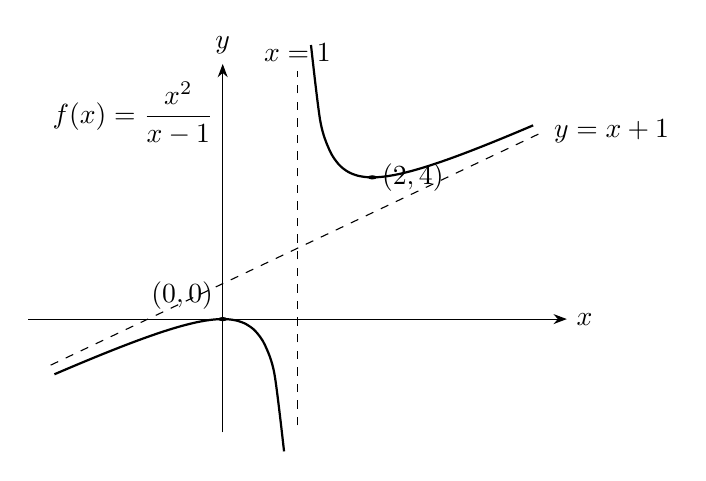
\begin{tikzpicture}[xscale=0.95,yscale=0.45,>=Stealth]
  \draw[->] (-2.6,0)--(4.6,0) node[right] {$x$};
  \draw[->] (0,-3.2)--(0,7.2) node[above] {$y$};
  \draw[dashed] (1,-3.0)--(1,7.0) node[above] {$x=1$};
  \draw[dashed] (-2.3,-1.3)--(4.3,5.3) node[right] {$y=x+1$};
  \draw[domain=-2.25:0.82,smooth,variable=\x,thick]
    plot ({\x},{\x+1+1/(\x-1)});
  \draw[domain=1.18:4.15,smooth,variable=\x,thick]
    plot ({\x},{\x+1+1/(\x-1)});
  \fill (0,0) circle (1.7pt) node[above left] {$(0,0)$};
  \fill (2,4) circle (1.7pt) node[right] {$(2,4)$};
  \node at (-1.2,5.8) {$f(x)=\dfrac{x^2}{x-1}$};
\end{tikzpicture}
\end{center}
% SOURCE-END U0110
}
\end{frame}
\typeout{MATH-AGENT-FRAME-END F072}
% FRAME-ID F073
\typeout{MATH-AGENT-FRAME-BEGIN F073}
\begin{frame}[t,fragile]{曲线的渐近线与函数图像}
\footnotesize
{\footnotesize
% SOURCE-BEGIN U0111 0 603
\begin{application}[凸性与机器学习优化]
	凸性在优化问题中非常重要。 直观地说，凸函数的图像没有“局部低谷冒充全局最低点”的现象。 在一元情形下，若 $f''(x)\ge0$，则 $f$ 为下凸函数；若严格凸且存在临界点，那么该临界点就是全局最小点。 许多基础机器学习模型，例如线性回归的均方误差损失，关于参数是凸函数，因此可以用导数和梯度方法稳定地寻找最优参数。
	
	\begin{example}
		设单样本线性模型损失为
		\[
		L(w)=\frac12(wx-y)^2,
		\]
		其中 $x,y$ 为常数。 讨论 $L$ 关于 $w$ 的凸性。
	\end{example}
	\begin{solution}
		对 $w$ 求导：
		\[
		L'(w)=x(wx-y),\qquad L''(w)=x^2\ge0.
		\]
		因此 $L$ 关于 $w$ 是下凸函数。 若 $x\neq0$，则 $L''(w)=x^2>0$，函数严格凸，唯一最小点由 $L'(w)=0$ 给出，即
		\[
		w=\frac{y}{x}.
		\]
		若 $x=0$，则 $L(w)=\frac12y^2$ 为常数函数，任意 $w$ 都是最小点。
	\end{solution}
	
\end{application}
% SOURCE-END U0111
}
\end{frame}
\typeout{MATH-AGENT-FRAME-END F073}
\section{泰勒公式}
% FRAME-ID F074
\typeout{MATH-AGENT-FRAME-BEGIN F074}
\begin{frame}[t,fragile]{目录}
\normalsize
{\color{black}\normalsize 1. 罗尔定理与拉格朗日中值定理\par}\vspace{0.22em}
{\color{black}\normalsize 2. 柯西中值定理与若干推论\par}\vspace{0.22em}
{\color{black}\normalsize 3. 洛必达法则\par}\vspace{0.22em}
{\color{black}\normalsize 4. 函数单调性判别法\par}\vspace{0.22em}
{\color{black}\normalsize 5. 函数的极值\par}\vspace{0.22em}
{\color{black}\normalsize 6. 函数的最值与应用优化\par}\vspace{0.22em}
{\color{black}\normalsize 7. 曲线的凸性与拐点\par}\vspace{0.22em}
{\color{black}\normalsize 8. 曲线的渐近线与函数图像\par}\vspace{0.22em}
{\color{blue}\normalsize 9. 泰勒公式\par}\vspace{0.22em}
\end{frame}
\typeout{MATH-AGENT-FRAME-END F074}
% FRAME-ID F075
\typeout{MATH-AGENT-FRAME-BEGIN F075}
\begin{frame}[t,fragile]{泰勒公式}
\footnotesize
\begin{block}{定理}
{\footnotesize
% SOURCE-BEGIN U0112 0 205
\textbf{泰勒公式：拉格朗日余项}\par

若 $f$ 在含 $x_0$ 与 $x$ 的区间上有 $n+1$ 阶连续导数，则存在介于 $x_0$ 与 $x$ 之间的 $\xi$，使得
\[
f(x)=\sum_{k=0}^{n}\frac{f^{(k)}(x_0)}{k!}(x-x_0)^k
+\frac{f^{(n+1)}(\xi)}{(n+1)!}(x-x_0)^{n+1}.
\]

% SOURCE-END U0112
}
\end{block}
\end{frame}
\typeout{MATH-AGENT-FRAME-END F075}
% FRAME-ID F076
\typeout{MATH-AGENT-FRAME-BEGIN F076}
\begin{frame}[t,fragile]{泰勒公式}
\footnotesize
{\footnotesize
\textbf{证明：}
% SOURCE-BEGIN U0113 0 271
记
\[
P_n(t)=\sum_{k=0}^{n}\frac{f^{(k)}(x_0)}{k!}(t-x_0)^k.
\]
固定 $x\neq x_0$，令
\[
R=f(x)-P_n(x),\qquad
M=\frac{R}{(x-x_0)^{n+1}}.
\]
构造
\[
F(t)=f(t)-P_n(t)-M(t-x_0)^{n+1}.
\]
由 $P_n$ 的构造可知
\[
F(x_0)=F'(x_0)=\cdots=F^{(n)}(x_0)=0,
\]
且由 $M$ 的定义，$F(x)=0$。
% SOURCE-END U0113
}
\end{frame}
\typeout{MATH-AGENT-FRAME-END F076}
% FRAME-ID F077
\typeout{MATH-AGENT-FRAME-BEGIN F077}
\begin{frame}[t,fragile]{泰勒公式（续1）}
\footnotesize
{\footnotesize
\textbf{证明：}
% SOURCE-BEGIN U0113 271 548
 对 $F$ 在以 $x_0,x$ 为端点的区间反复使用罗尔定理：由 $F(x_0)=F(x)=0$，存在一点使 $F'=0$；又 $F'(x_0)=0$，可在相应子区间再次使用罗尔定理，逐次得到存在 $\xi$ 介于 $x_0$ 与 $x$ 之间，使
\[
F^{(n+1)}(\xi)=0.
\]
而
\[
F^{(n+1)}(t)=f^{(n+1)}(t)-M(n+1)!.
\]
故
\[
M=\frac{f^{(n+1)}(\xi)}{(n+1)!}.
\]
代回 $R=M(x-x_0)^{n+1}$，得泰勒公式。

% SOURCE-END U0113
}
\end{frame}
\typeout{MATH-AGENT-FRAME-END F077}
% FRAME-ID F078
\typeout{MATH-AGENT-FRAME-BEGIN F078}
\begin{frame}[t,fragile]{泰勒公式}
\normalsize
\begin{block}{定理}
{\normalsize
% SOURCE-BEGIN U0114 0 284
\textbf{泰勒公式：皮亚诺（Peano）余项}\par

若 \(f\) 在 \(x_0\) 的某邻域内有定义，并且在 \(x_0\) 处具有直到 \(n\) 阶的导数，则当 \(x\to x_0\) 时，
\[
f(x)=\sum_{k=0}^{n}\frac{f^{(k)}(x_0)}{k!}(x-x_0)^k
+o\bigl((x-x_0)^n\bigr).
\]
这里的 \(o((x-x_0)^n)\) 表示余项除以 \((x-x_0)^n\) 后趋于 \(0\)。与拉格朗日余项相比，皮亚诺余项直接描述局部渐近阶，特别适合计算极限。

% SOURCE-END U0114
}
\end{block}
\end{frame}
\typeout{MATH-AGENT-FRAME-END F078}
% FRAME-ID F079
\typeout{MATH-AGENT-FRAME-BEGIN F079}
\begin{frame}[t,fragile]{泰勒公式}
\normalsize
\begin{block}{例题}
{\normalsize
% SOURCE-BEGIN U0115 0 78
\textbf{麦克劳林（Maclaurin）公式}\par

写出 $\ee^x,\sin x,\ln(1+x)$ 在 $0$ 处到常用阶数的展开。

% SOURCE-END U0115
}
\end{block}
\pause
{\normalsize
\textbf{解：}
% SOURCE-BEGIN U0116 0 313
\[
\ee^x=1+x+\frac{x^2}{2!}+\cdots+\frac{x^n}{n!}+o(x^n).
\]
\[
\sin x=x-\frac{x^3}{3!}+\frac{x^5}{5!}+\cdots+(-1)^m\frac{x^{2m+1}}{(2m+1)!}+o(x^{2m+1}).
\]
\[
\ln(1+x)=x-\frac{x^2}{2}+\frac{x^3}{3}-\cdots+(-1)^{n-1}\frac{x^n}{n}+o(x^n).
\]
这些公式是皮亚诺余项形式的泰勒公式在 \(x_0=0\) 时的应用。以 \(0\) 为展开点的泰勒公式也称为麦克劳林公式。

% SOURCE-END U0116
}
\end{frame}
\typeout{MATH-AGENT-FRAME-END F079}
% FRAME-ID F080
\typeout{MATH-AGENT-FRAME-BEGIN F080}
\begin{frame}[t,fragile]{泰勒公式}
\normalsize
\begin{block}{例题}
{\normalsize
% SOURCE-BEGIN U0117 0 84
\textbf{极限}\par

求 $\displaystyle\lim_{x\to0}\frac{\cos x-1+\frac{x^2}{2}}{x^4}$。

% SOURCE-END U0117
}
\end{block}
\pause
{\normalsize
\textbf{解：}
% SOURCE-BEGIN U0118 0 184
由泰勒展开
\[
\cos x=1-\frac{x^2}{2}+\frac{x^4}{24}+o(x^4).
\]
故分子为
\[
\left(1-\frac{x^2}{2}+\frac{x^4}{24}+o(x^4)\right)-1+\frac{x^2}{2}
=\frac{x^4}{24}+o(x^4).
\]
因此极限为 $1/24$。

% SOURCE-END U0118
}
\end{frame}
\typeout{MATH-AGENT-FRAME-END F080}
% FRAME-ID F081
\typeout{MATH-AGENT-FRAME-BEGIN F081}
\begin{frame}[t,fragile]{泰勒公式}
\normalsize
\begin{block}{例题}
{\normalsize
% SOURCE-BEGIN U0119 0 84
\textbf{用泰勒判别极值}\par

设 $f'(x_0)=f''(x_0)=0$，$f^{(3)}(x_0)\neq0$。 证明 $x_0$ 不是极值点。

% SOURCE-END U0119
}
\end{block}
\pause
{\normalsize
\textbf{解：}
% SOURCE-BEGIN U0120 0 267
由泰勒公式，
\[
f(x)=f(x_0)+\frac{f^{(3)}(x_0)}{3!}(x-x_0)^3+o((x-x_0)^3).
\]
记 $A=f^{(3)}(x_0)/6\neq0$。 则
\[
f(x)-f(x_0)=(x-x_0)^3[A+o(1)].
\]
当 $x$ 足够接近 $x_0$ 时，$A+o(1)$ 与 $A$ 同号。 而 $(x-x_0)^3$ 在 $x_0$ 两侧异号，所以 $f(x)-f(x_0)$ 在两侧异号。 因此 $f(x_0)$ 既不是局部极大值，也不是局部极小值。

% SOURCE-END U0120
}
\end{frame}
\typeout{MATH-AGENT-FRAME-END F081}
% FRAME-ID F082
\typeout{MATH-AGENT-FRAME-BEGIN F082}
\begin{frame}[t,fragile]{泰勒公式}
\normalsize
{\normalsize
% SOURCE-BEGIN U0121 0 497
\begin{application}[工程与物理：小角度近似的误差]
第4章由重要极限知道 $\sin\theta\approx\theta$（$\theta$ 必须用弧度）。现在用已建立的泰勒公式进一步说明误差：
\[
\sin\theta=\theta-\frac{\theta^3}{6}+O(\theta^5),
\qquad
\sin\theta-\theta=-\frac{\theta^3}{6}+O(\theta^5).
\]
因此主要误差是三阶量。用 $|\theta^3|/6$ 估计其量级：
\[
\begin{array}{c|ccc}
\theta&0.1&0.2&0.5\\ \hline
|\theta|^3/6&1.67\times10^{-4}&1.33\times10^{-3}&2.08\times10^{-2}
\end{array}
\]
角度减半时，主要误差约缩小到原来的 $1/8$。这一结论可用于理解小振幅单摆或近轴光学中的线性化，但近似是否足够精确仍取决于具体问题允许的误差。
\end{application}
% SOURCE-END U0121
}
\end{frame}
\typeout{MATH-AGENT-FRAME-END F082}
% FRAME-ID F083
\typeout{MATH-AGENT-FRAME-BEGIN F083}
\begin{frame}[t,fragile]{参考文献}
\normalsize
{\normalsize
% SOURCE-BEGIN U0123 0 205
\begin{thebibliography}{99}
\bibitem{TaizPlant} TAIZ L, ZEIGER E, M{\o}LLER I M, et al. \emph{Plant Physiology and Development}（6th ed.）[M]. Sunderland, MA: Sinauer Associates, 2015.
\end{thebibliography}
% SOURCE-END U0123
}
\end{frame}
\typeout{MATH-AGENT-FRAME-END F083}
\end{document}
